\documentclass[class=report, crop=false, a4paper, 12pt]{standalone}

%Packages import
\usepackage{../pkgs}


\begin{document}
\newpage
% A face recognition system works in either or both of two modalities: face verification (or authentication) or face identification (or recognition). The difference between them lies in the final stage of the workflow, identification involves a one-to-one pairing, while identification is a one-to-many match.

\section{Face Recognition - Theory Background}
Face Recognition (FR) is a thoroughly debated and extensively researched task in the Computer Vision community for more than two decades~\autocite{ranjanDeepLearningUnderstanding2018}, popularized in the early 1990s with the introduction of the Eigenfaces~\autocite{turkEigenfacesRecognition1991} or Fisherfaces~\autocite{p.n.belhumeurEigenfacesVsFisherfaces1997} approaches. These methods projected faces in a low-dimensional subspace assuming certain distributions, but lacked the ability to handle uncontrolled facial changes that broke said assumptions, henceforth, bringing about face recognition approaches through local-features~\autocite{chengjunliuGaborFeatureBased2002, ahonenFaceDescriptionLocal2006} that, even though, presented considerable results, weren't distinctive or compact. Beginning in 2010, methods based on learnable filters arose~\autocite{z.caoFaceRecognitionLearningbased2010,leiLearningDiscriminantFace2014}, but unfortunately revealed limitations when nonlinear variations were at stake.

\par Earlier methods for FR worked appropriately when the data was handpicked or generated on a constrained environment, however, they didn't scale adequately in the real world were there are large fluctuations in, particularly, pose, age, illumination, background scenario, the presence of facial occlusion~\autocite{ranjanDeepLearningUnderstanding2018} and many unimaginable more \autocite{kalkaIJBIARPAJanus2018}. These shortcomings can be dealt with by using Deep Learning, a framework of techniques that solves the nonlinear inseparable classes problem \red{ref.}, more specifically a structure called Convolutional Neural Network (CNN)~\autocite{wangDeepFaceRecognition2021}. 

\par CNNs are an Artificial Neural Network (ANN) that exhibit a better performance on image or video-based tasks compared to other methods~\autocite{lecunGradientBasedLearningApplied1998}. They were greatly hailed in 2012, after the AlexNet~\autocite{krizhevskyImageNetClassificationDeep2012} victory, by a great margin, in the ImageNet Large Scale Visual Recognition Challenge (ILSVRC). Just two years later, DeepFace~\autocite{taigmanDeepFaceClosingGap2014} revolutionized the benchmarks scores by achieving state-of-the-art results that approached human performance, reinforcing even further the importance of Deep Learning and shifting the research path to be taken~\autocite{wangDeepFaceRecognition2021}.

\par Given what has been stated so far and the proven robustness, performance, and overall results in computer vision \red{ref. won competitions}, the methods discussed in this dissertation will therefore deal exclusively with Deep Learning approaches. For more information on other methods, please refer to~\autocite{learned-millerLabeledFacesWild2016}.
% The exponential growth in the Artificial Intelligence domain, its corresponding subfields and technologies involved, spanned a plethora of terms that can be easily confused, mistook or mixed. For a better understanding of this dissertation, before discussing methods and implementations, it's important to analyze the fundamentals.


% \vspace{0.7\baselineskip}
% \noindent\textbf{$\rightarrow$ Computer Vision} is the science of trying to mimic with a computer what the humans do when looking at a scene, that is, extracting information from images through a series of computational techniques.~\autocite{szeliskiComputerVisionAlgorithms2022}

% \vspace{0.7\baselineskip}
% \noindent\textbf{$\rightarrow$ Image querying}, is the process of finding information in a database of images that corresponds to the user query\footnote{Query, in computer science, is the request for information in a database.}, in this case, an image query\autocite{bartoliniImageQuerying2009}.  

\subsection{Convolutional Neural Networks}
\begin{figure}[!h]
    \centering
    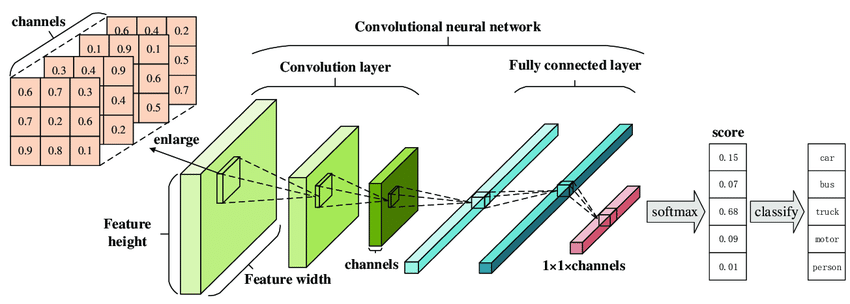
\includegraphics[width=0.85\textwidth]{Architecture-of-a-Convolutional-Neural-Network-CNN-The-traditional-CNN-structure-is.png}
    \caption{Architecture of a Convolutional Neural Network~\autocite{kangDeepSimilarityMetric2019}.}
    \label{fig:cnn}
\end{figure}


\par There are several types of Neural Networks architectures, but Convolutional Neural Networks (CNNs or ConvNets) are probably the most widely implemented model overall~\autocite{yamashitaConvolutionalNeuralNetworks2018, liSurveyConvolutionalNeural2022}. Using CNNs for Computer Vision tasks~\autocite{krizhevskyImageNetClassificationDeep2012,taigmanDeepFaceClosingGap2014,tompsonEfficientObjectLocalization2015, zhangImprovedBreastCancer2021}, in this specific case, Face Recognition, is not an arbitrary choice, but due to the fact that the network design benefits from the intrinsic characteristics of the input data: images have an array-like structure~\autocite{yamashitaConvolutionalNeuralNetworks2018}, and local groups of values are correlated (motifs or patterns) and invariant to spatial location~\autocite{lecunDeepLearning2015,caoReviewNeuralNetworks2018}. Furthermore, when compared to fully connected networks, CNNs are superior due to 4 key features: 1) Shared weights between the same features in different locations reduce the number of parameters~\autocite{liSurveyConvolutionalNeural2022}, 2) sparse connections~\autocite{alzubaidiReviewDeepLearning2021}, 3) pooling layers and 4) automatically identifies the relevant features without any human supervision~\autocite{alzubaidiReviewDeepLearning2021,liSurveyConvolutionalNeural2022}.
% \begin{enumerate}
%     \item Designed to process multidimensional arrays~\autocite{lecunDeepLearning2015};
%     \item Shared weights between the same features in different locations; %Invariance to shift, distortions and rotations
%     \item Automatically identifies the relevant features without any human supervision, hence, small amounts of preprocessing~\autocite{alzubaidiReviewDeepLearning2021,liSurveyConvolutionalNeural2022}; %Easier to train
%     \item Sparse connections~\autocite{alzubaidiReviewDeepLearning2021}; %Less complexity, easier to train; %Invariance to shift, distortions and rotations and less network complexity (easier to train)
%     \item Pooling layers reduce the spatial size of the input data. %Invariance to shift, distortions and rotations
% \end{enumerate}
% Check this article for better description of key features~\autocite{liSurveyConvolutionalNeural2022}

% The ensemble of features 2, 4 and 5 enable an invariance of the network to small shifts, distortions and rotations~\autocite{guRecentAdvancesConvolutional2018,lecunDeepLearning2015}, while 2, 3, 4 and 5 helps to reduce the complexity of the model, and as a result training it is easier~\autocite{guRecentAdvancesConvolutional2018,liSurveyConvolutionalNeural2022}.

\par In the CNN category itself there are different variants, but they all abide the fundamental structure of a feedforward hierarchical multi-layer network \reffig{fig:cnn}. Feedforward because the information only flows in a singular direction without cycling~\autocite{zellSimulationNeuronalerNetze1994}, hierarchical because the higher complexity internal representations are learned from lower ones~\autocite{lecunDeepLearning2015, zhuBCNNBranchConvolutional2017} and multi-layer because it is composed of a series of stages, blocks or layers. The raw data is fed to an input layer, forwarded to a sequence of intercalating convolutional and pooling layers, transmitted to a stage of one or more fully-connected layers~\autocite{lecunDeepLearning2015, guRecentAdvancesConvolutional2018, alzubaidiReviewDeepLearning2021}.   

\subsubsection{Convolutional Layer}
\par The convolutional layer aims at extracting feature representations from the inputs, and is formed by a set of learnable filters called \textbf{kernels} and an \textbf{activation function}~\autocite{guRecentAdvancesConvolutional2018,yamashitaConvolutionalNeuralNetworks2018}. 

\begin{figure}[!h]
    \centering
    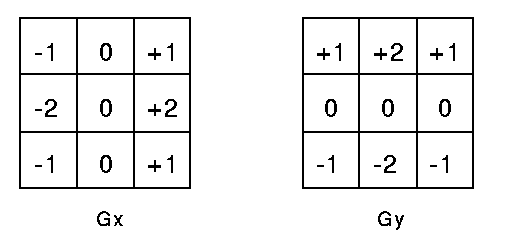
\includegraphics[width=0.45\textwidth]{sobel.png}
    \caption{3x3 Kernels of the Sobel-Feldman operator used for edge detection~\autocite{sobelIsotropicGradientOperator1973}.}
    \label{fig:sobel}
\end{figure}

A \textbf{kernel}\footnote{Or feature detector~\autocite{ajitReviewConvolutionalNeural2020}.} \reffig{fig:sobel}, is a grid-like structure of fixed dimensions [WxHxD], where W is the width and H is the height. The dimension D relates to the depth of the kernel and is used to multichannel images, such as RGB ones (3 channels). Each of its elements is a learnable weight that is adjusted during training to extract significant features~\autocite{alzubaidiReviewDeepLearning2021}. 

\begin{figure}[!h]
    \centering
    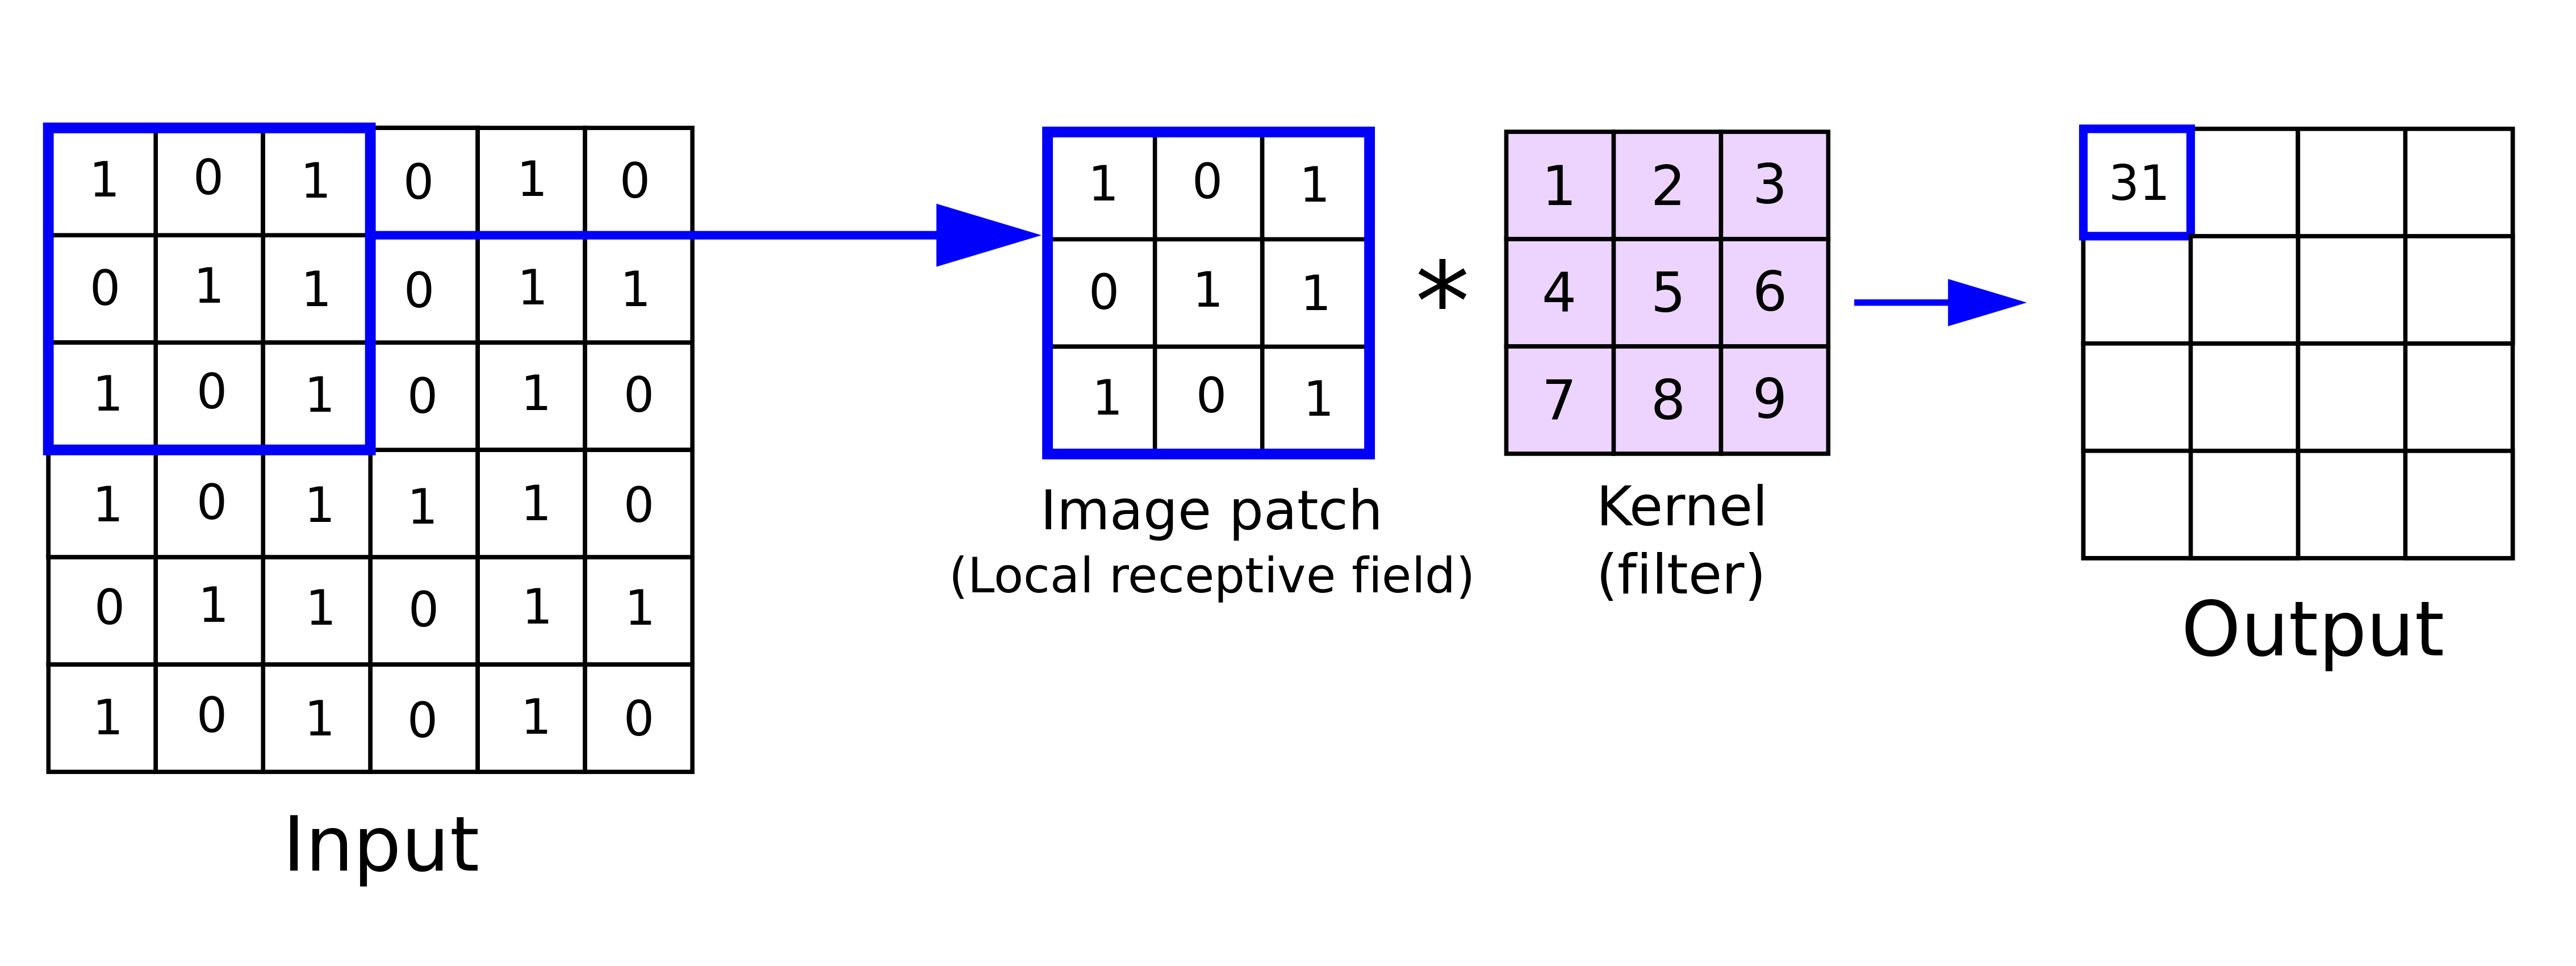
\includegraphics[width=0.7\textwidth]{conv.png} %source: https://anhreynolds.com/blogs/cnn.html
    \caption{Convolution}
    \label{fig:conv}
\end{figure}

\par With a predetermined \textbf{stride}, the kernel scans its receptive field~\autocite{khanSurveyRecentArchitectures2020}, horizontally and vertically, through the input data, and produces the feature map\footnote{Also referred to as feature representation~\autocite{liSurveyConvolutionalNeural2022} or activation map~\autocite{ajitReviewConvolutionalNeural2020}.}~\autocite{lecunDeepLearning2015, alzubaidiReviewDeepLearning2021} by performing an element-wise product, called \textbf{convolution} \reffig{fig:conv}, that can be described as follows~\autocite{khanSurveyRecentArchitectures2020}:
$$
f_l^k(p, q) = \sum_{c}^{}\sum_{x, y}^{}i_c(x, y)\cdot w^k_l(u,v)
$$
where $f_l^k(p, q)$ is an element at line $p$ and column $q$ in the feature map from the k-th kernel in the l-th layer, $i_c(x, y)$ is the element at line $x$ and row $y$ in the input data, and $w^k_l(u,v)$ is the weight at line $u$ and column $v$ from the k-th kernel of the l-th layer. 

% To adjust the density of the convolution, the value of the \textbf{stride}, which represents the shift between convolutions, is modified~\autocite{ajitReviewConvolutionalNeural2020,liSurveyConvolutionalNeural2022}.

\begin{figure}[!h]
    \centering
    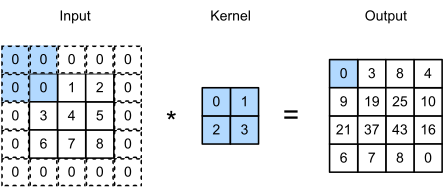
\includegraphics[width=0.6\textwidth]{padding.png} %source: https://d2l.ai/chapter_convolutional-neural-networks/padding-and-strides.html
    \caption{Convolution}
    \label{fig:padding}
\end{figure}

\par At the edge of the input, it's not possible to overlap the whole kernel over all the elements, reaching a point where it can't shift anymore, so the dimensions of the feature map would be unintentionally reduced and information would be lost. Therefore, as seen in \reffig{fig:padding}, usually \textbf{zero padding} is employed to solve the aforesaid problems~\autocite{yamashitaConvolutionalNeuralNetworks2018}.

\par The overall architecture of CNNs are inspired by the visual perception~\autocite{hubelReceptiveFieldsBinocular1962}, so a direct parallelism can be made to better define the \textbf{activation function}. The kernels can be seen as receptors, or artificial neurons, that respond to different features, whereas the activation function is a simulation of the threshold function that dictates if the next neuron is activated or not. Additionally, the convolution operation is linear, consequently, if no nonlinear activation function was used, the input of the next layer would be a linear output of the previous layer. The introduction of nonlinearity through activation functions, such as ReLU (Rectified Linear Unit) and its variations (Leaky, Parametric, Randomized, Concatenated, Bounded, etc) or others like Sigmoid or Tanh \autocite{dubeyActivationFunctionsDeep2022}, allows deep neural networks to approximate any function, enhancing the ability to fit to any data~\autocite{liSurveyConvolutionalNeural2022}.

\subsubsection{Pooling Layer}
After the features are extracted, the spatial location of them become less relevant for the following layers. Introducing a pooling layer with the purpose of reducing the spatial size of the feature maps by joining identical features~\autocite{lecunDeepLearning2015, guRecentAdvancesConvolutional2018}, then only the dominant response will prevail. This downsampling operation has two important advantages that help reduce the overfitting problem~\autocite{ajitReviewConvolutionalNeural2020,liSurveyConvolutionalNeural2022}. First, it reduces the number of learnable features, which requires less memory to train the network. Second, it enhances feature extraction invariance to shifts and rotations by emphasizing only the relevant features.

\begin{figure}[!h]
    \centering
    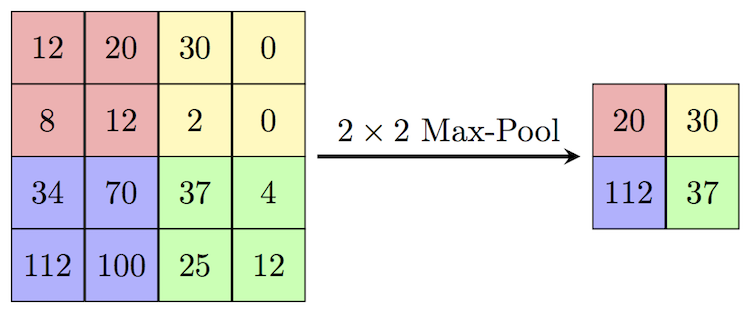
\includegraphics[width=0.6\textwidth]{maxpool.png} %source: https://paperswithcode.com/method/max-pooling
    \caption{Max pool}
    \label{fig:maxpool}
\end{figure}

There are many ways of downsampling the feature map through pooling such as min pooling, average pooling or stochastic pooling, however max pooling is by far the most popular one. As pictured in \reffig{fig:maxpool}, this operation divides the feature map in sections and computes the maximum value in each while discarding the other ones.

\subsubsection{Fully Connected Layer}
The fully connected (FC) layer is located at the end of the network. It is a dense, feedforward neural network in which every neuron is connected to all other neurons~\autocite{yamashitaConvolutionalNeuralNetworks2018, alzubaidiReviewDeepLearning2021}. The final feature map is flattened and transformed in a one-dimensional feature vector and the purpose of the FC layer is using this vector as an input, and act as the CNN classifier by performing high logic reasoning~\autocite{guRecentAdvancesConvolutional2018}.

\subsection{Training}
Training a network in the context of CNNs is the process of finding the optimal kernel weights' values. The training data is passed through the model, the predictions asserted and the distance between them and the expected ones is measured by a loss function. LeCun \textit{et al.}~\autocite{lecunGradientBasedLearningApplied1998} presents the problem as follows:
$$
E^p = \mathcal{D}(D^p, Y^p)
$$

\noindent The loss function, $E^p$, is a measure of error. It computes the difference between the expected result, $D^p$, and the predicted result $Y^p$, where $Y^p = F(Z^p, W)$ is a function of the $p$-th training example, $Z^p$, for a determined weight $W$. Additionally, $E_{train}(W)$, is the average of all the errors calculated in a training set $\left\{(Z^x, D^x),\dots (Z^p, D^p)\right\}$. Training the network is nothing more than a function minimization problem, and for that there are several techniques, the \textbf{optimizers}.

\subsubsection{Optimizers}

\begin{figure}[!h]
    \centering
    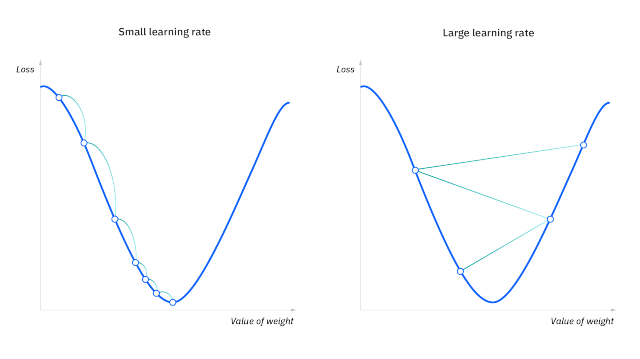
\includegraphics[width=0.6\textwidth]{gd.png} %source: https://www.ibm.com/topics/gradient-descent
    \caption{Gradient descent}
    \label{fig:gd}
\end{figure}


\par By computing the gradient of the loss function in respect to the learnable parameters it allows studying how said parameters influence the loss function and how it can be more efficiently minimized. This algorithm is called \textbf{gradient descent}~\autocite{ruderOverviewGradientDescent}, and is the simplest minimization technique. By definition, the gradient of a function is the direction of the steepest ascent, henceforth, the learnable parameters are updated once every epoch in the opposite direction to reduce the error: 
$$
W_k = W_{k-1}-\epsilon\frac{\delta E(W)}{{\delta} W}
$$
\noindent where $\epsilon$ is a constant called \textbf{learning rate} that controls how much the parameters are updated and has an immense impact in the performance of a neural network \reffig{fig:gd}. According to Goodfellow \textit{et al.}~\autocite{Goodfellow-et-al-2016}, if the learning rate is set too low, training will be much slower and can become permanently stuck with a high training error. On the other hand, if the learning rate is too high, the gradient descent can increase the training error instead of reducing it.
\par \textbf{Stochastic Gradient Descent} (SGD)~\autocite{alzubaidiReviewDeepLearning2021} is the algorithm of choice to optimize the loss function and its main difference is that the parameters updating routine. First, training samples are randomly sampled in every epoch, then the gradient is calculated for each at a time, and, finally, the parameters are updated accordingly. This is an efficient algorithm in terms of memory usage, but, since the updates occur once at every sample, the convergence can be noisy. Other optimizers worth of mentioning are: \textbf{1) Mini-batch Gradient Descent} - divides the training data into non-overlapping batches and the parameters are updated on each one of them; \textbf{2) Momentum}~\autocite{polyakMethodsSpeedingConvergence1964} - introduces a new hyperparameter to the network called momentum, that accumulates previous gradients, that accelerates the optimizer in the correct direction of minimization and reduces error's oscillation during optimization; \textbf{3) Adam (Adaptive moment estimation)}~\autocite{kingmaAdamMethodStochastic2015} - uses the first and second moments of the gradients (gradient's mean and variance, respectively) to better optimize the parameters.

\subsubsection{Backpropagation}
\par Regardless of the optimizer selected, computing an analytical expression for the gradient is trivial, but evaluating it is a computational heavy task when the aim is to find a minimum with respect to all the parameters in the network. To this extent, the backpropagation (or backprop) algorithm is a solution to do so efficiently~\autocite{6795724}. Backprop is usually referred to as a training algorithm, but that is not true. Backpropagation is not a training algorithm, it is simply the method of computing the gradient using a fixed sequence, efficient application of the \textit{Chain Rule of Calculus} $\left(\frac{dz}{dx} = \frac{dz}{dy}\frac{dy}{dx}\right)$, considering that it starts at the final layer, and proceeding backwards~\autocite{Goodfellow-et-al-2016}. 

\phantomsection\label{transf learning}
\subsubsection{Transfer Learning} %Source: https://cs231n.github.io/transfer-learning/
\par Developing a Deep Learning system requires data in large scale~\autocite{parkhiDeepFaceRecognition2015}, specially labeled one. In a general sense, gathering information can be very difficult, but if the domain of study is too specific or not widespread enough, that poses an even bigger challenge. To overcome this solution, based on the psychologist C.H. Judd's theory, a technique called Transfer Learning takes place. It is defined by Zhuang \textit{et al.}~\autocite{zhuangComprehensiveSurveyTransfer2020} as: given a source and target domain, transfer learning is the act of utilizing the knowledge acquired in the source to further improve the performance of the learned decision functions on the target domain. A classic example is the case of learning how to ride a motorcycle. It will be easier for someone who has already learned how to ride a bicycle than it is to someone starting from scratch.
\par In the context of CNNs, there are 2 ways of approaching the aforesaid problem. By taking a pre-trained CNN and either use it as a fixed feature extractor or fine-tune it. In the first case, an already trained CNN is used, however, the final few layers or the fully connected one is discarded and retrained to a specific task, while the rest of the network is frozen and used as the feature extractor that will feed the classifier input. The second approach is referred to as fine-tuning a network and, as the name suggests, the source network's parameters are used as a starting point and is entirely retrained using the desired data. It is also common to freeze the first layers since they are responsible to extract the more general, universal features (edges or patterns).


\newpage
\section{A Face Recognition System}

\begin{figure}[!h]
    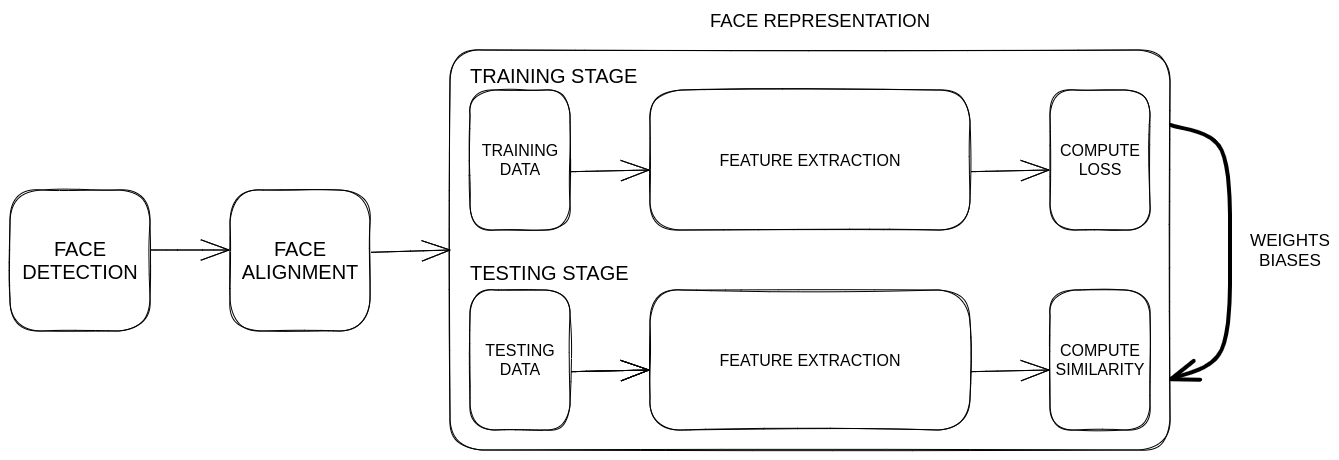
\includegraphics[scale=0.30]{fr_pipeline.png}
    \caption[Pipeline]{A typical face recognition pipeline, guided by the approach in~\autocite{wangDeepFaceRecognition2021}.}
    \label{fig:fr pipeline}
\end{figure}

\par According to Ranjan \textit{et al.}~\autocite{ranjanDeepLearningUnderstanding2018}, the goal of a FR system is to find, process and learn from a face, gathering as much information as possible, and as a result, it is one of the most widely implemented biometric system solutions in light of its versatility when facing real world application~\autocite{duElementsEndtoendDeep2022}.

\par By and large, all end-to-end automatic face recognition systems follow a sequential and modular\footnote{Sequential because each stage relies on the output from the previous ones, and modular in the sense that each stage employs its own method and it can be modified to better adapt to specific tasks.} pipeline \reffig{fig:fr pipeline} composed of three pillar stages~\autocite{wangDeepFaceRecognition2021}: face detection, face alignment and face representation. First an image or video feed is used as an input then, as the name suggests, the \textbf{face detection} module is responsible for finding a face. Next, the \textbf{face alignment} phase applies spatial transformations to the data in order to normalize the faces' pictures (or frames, in the case where a video is used) to a standardized view. Finally, the \textbf{face representation} stage, makes use of deep learning techniques to learn and further extract discriminative features that will allow the recognition \textit{per se}. A feature is nothing more than a characteristic inherent to the input image, it can be "something" or a collection of, that has been measured or processed, and presented as a result~\autocite{Goodfellow-et-al-2016}.

\par All three stages have their individual importance and methods of implementation\footnote{For a deeper and extensive study, please refer to:~\autocite{zafeiriouSurveyFaceDetection2015} in the case of classic face detection approaches and~\autocite{minaeeGoingDeeperFace2021} for deep learning based methods;~\autocite{wangFacialFeaturePoint2018} addresses traditional face alignment methods and is complemented with~\autocite{duElementsEndtoendDeep2022} for more up-to-date techniques; and~\autocite{learned-millerLabeledFacesWild2016} tackles classic face representation.}. \textbf{Face detection} is achievable through classical approaches~\autocite{violaRapidObjectDetection2001, brubakerDesignCascadesBoosted2008} or deep methods, among them is~\autocite{dengRetinaFaceSinglestageDense2019} and the widely applied~\autocite{zhangJointFaceDetection2016a}. \textbf{Face alignment}, once again, can be accomplished through traditional measures~\autocite{cootesViewbasedActiveAppearance2002, martinezLocalEvidenceAggregation2013} or more modern ones, namely~\autocite{huangPropagationNetPropagatePoints2020} or the aforementioned~\autocite{zhangJointFaceDetection2016a} which concurrently performs detection and alignment. To conclude, the \textbf{face representation} module is no exception, and can also be divided in two groups, regarding the methodology used. Some conventional systems were already mentioned, such as~\autocite{p.n.belhumeurEigenfacesVsFisherfaces1997,turkEigenfacesRecognition1991}, and the deep learning ones are the object of discussion of this dissertation and will be reviewed along the following sections, therefore, the focus will be on describing, with particular interest, the face representation stage.

\subsection{Face Detection}
\par Face detection is the first step in any automatic facial recognition system. Given an input image to a face detector module, it is in charge of detecting every face in the picture and returning bounding-boxes coordinates, for each one, with a certain confidence score~\autocite{duElementsEndtoendDeep2022,ranjanDeepLearningUnderstanding2018}.

\par Previously employed traditional face detectors are incapable of detecting facial information when faced with challenges such as variants in image resolution, age, pose, illumination, race, occlusions or accessories (masks, glasses, makeup)~\autocite{duElementsEndtoendDeep2022,ranjanDeepLearningUnderstanding2018}. The progress in deep learning and increasing GPU power led DCNNs to become a viable and reliable option that solves said problems in face detection. 

\par These techniques can be included in different categories. A more analytical perspective~\autocite{duElementsEndtoendDeep2022} distributes the methods, depending upon their architecture or purpose of application, over seven categories: multi-stage, single-stage, anchor-based, anchor-free, multi-task learning, CPU real-time and, finally, problem-oriented. Additionally, being as the face detection problem can be seen as a specific task in a general object detection situation, it is no surprise that several works inherit from them and, therefore, some bases are referenced throughout the next list.

\vspace{0.5\baselineskip}
\begin{figure}[h!]
    \centering
    \begin{minipage}[c]{0.38\textwidth}
      \centering
      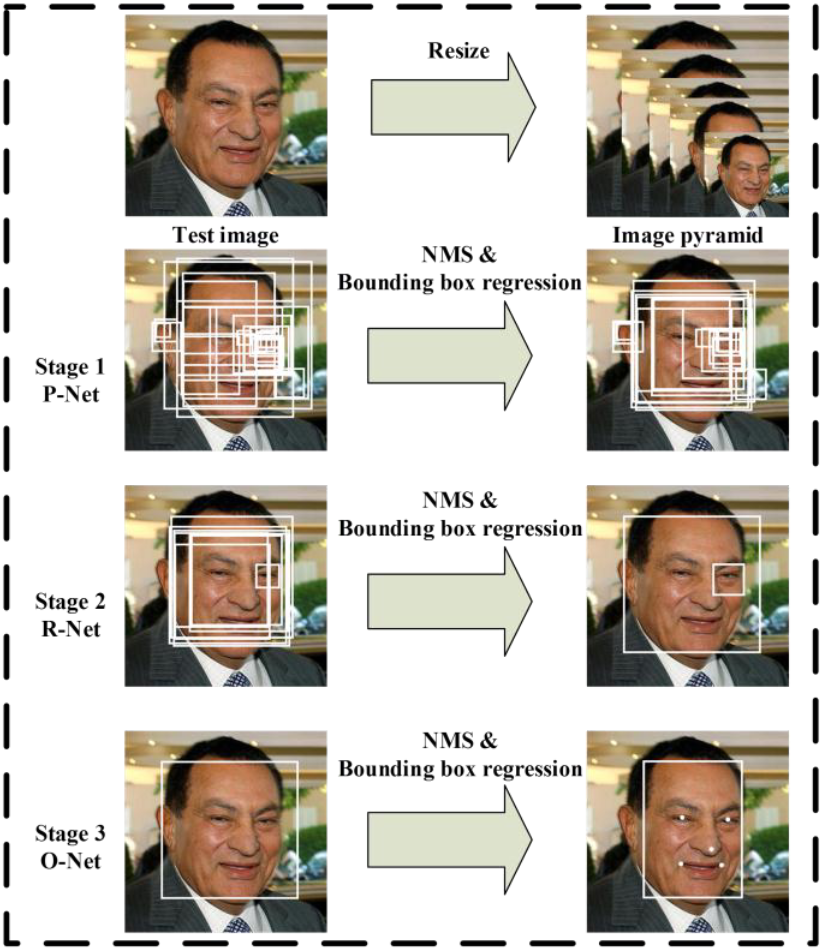
\includegraphics[width=\textwidth]{mtcnn.png}
      \label{fig:mtcnn}
    \end{minipage}
    \hspace{0.5cm}
    \begin{minipage}[c]{0.52\textwidth}
      \centering
      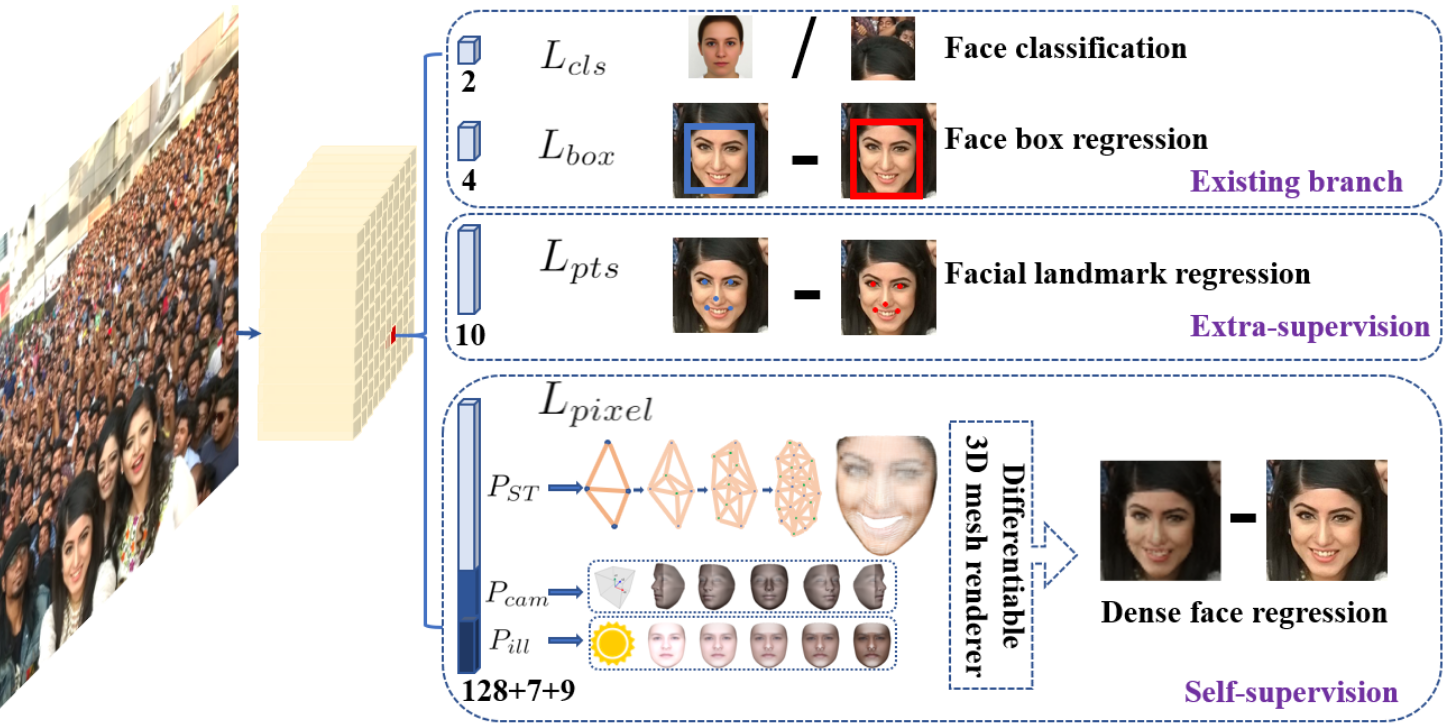
\includegraphics[width=\textwidth]{retinaface.png}
      \label{fig:retinaface}
    \end{minipage} 
    \begin{minipage}{0.4\textwidth}
        \vspace{-0.5cm}
        \centering
        \footnotesize a)
    \end{minipage}
    \hfill
    \begin{minipage}{0.4\textwidth}
        \vspace{-0.5cm}
        \centering
        \footnotesize b)
    \end{minipage}
    \vspace{-0.4cm}
    \caption{Comparison between \textbf{a)} MTCNN: multi-stage, CPU real-time and multi-task learning, and \textbf{b)} RetinaFace: single-stage, anchor-based, CPU real-time and multi-task learning. MTCNN~\autocite{zhangJointFaceDetection2016a} proposes a series of bounding boxes then, through a series of refinement stages, the best solution and landmarks are found. RetinaFace~\autocite{dengRetinaFaceSinglestageDense2019} accomplishes, in a single-stage, face classification and bounding box regression by evaluating anchors, landmark localization and dense 3D projection for facial correspondence.}
    \label{fig:mtcnn vs retinaface}
\end{figure}
  

\noindent\textbf{$\rightarrow$ Multi-stage} methods~\autocite{dengRetinaFaceSinglestageDense2019} include all the coarse-to-fine facial detectors that work in similar manner to the following two phases. First, bounding box proposals are generated by sliding a window through the input. Then, over one or several subsequent stages, false positives are rejected and the approved bounding boxes are refined. To complement, one widely applied object detection protocol that inspired face detection methods and perfectly describes the steps mentioned above is Faster R-CNN~\autocite{renFasterRCNNRealTime2016}. However, these methods can be slower and have a more complex way of training~\autocite{xuCenterFaceJointFace2019}.

\vspace{0.7\baselineskip}
\noindent\textbf{$\rightarrow$ Single-stage} approaches~\autocite{dengRetinaFaceSinglestageDense2019} are the ones that perform classification and bounding box regression without the necessity of a proposal stage, producing highly dense face locations and scales. This structure takes inspiration, once again, from general object detectors, for example, the Single Shot MultiBox detector, commonly referred to as SSD~\autocite{liuSSDSingleShot2016}. Finally, the methods included in this class are more efficient, but can incur in compromised accuracy, when compared to multi-stage.

\vspace{0.7\baselineskip}
\noindent\textbf{$\rightarrow$ Anchor-based} techniques~\autocite{liuHAMBoxDelvingOnline2019, dengRetinaFaceSinglestageDense2019, zhangFaceDetectionUsing2018} detect faces by predefining anchors with different settings (scales, strides, number, etc.) on the feature maps, then performing classification and bounding box regression on them until an acceptable output is found. As proven by Liu and Tang \textit{et al.}~\autocite{liuHAMBoxDelvingOnline2019}, the choice of anchors highly influences the results of prediction. Hence, it is necessary to fine-tune them on a situation-by-situation basis, otherwise, there is a limitation in generalization. Furthermore, higher densities of anchors directly generate an increase in computational overhead.

\vspace{0.7\baselineskip}
\noindent\textbf{$\rightarrow$ Anchor-free} procedures, obviously, do not need predefined anchors in order to find faces. Alternatively, these methods address the face detection by using different techniques. For example, DenseBox~\autocite{huangDenseBoxUnifyingLandmark2015} which attempts to predict faces by processing each pixel as a bounding box, or CenterFace~\autocite{xuCenterFaceJointFace2019} that treats face detection as a key-point estimation problem by predicting the center of the face and bounding boxes. Even so, relating to the accuracy of anchor-free approaches, there's still room for improvement for false positives and stability in the training stage~\autocite{duElementsEndtoendDeep2022}.

\vspace{0.7\baselineskip}
\phantomsection\label{mt learning}
\noindent\textbf{$\rightarrow$ Multi-task learning} are all the methodologies that conjointly performs other tasks, namely facial landmark\footnote{A facial landmark is a key-point in a face that contributes with important geometric information, namely the eyes, nose, mouth, etc.~\autocite{fengWingLossRobust2018}} localization, during face classification and bounding box regression~\autocite{duElementsEndtoendDeep2022}. CenterFace~\autocite{xuCenterFaceJointFace2019} is one example, and so it is the widely implemented MTCNN~\autocite{zhangJointFaceDetection2016a}, which correlated bounding boxes and face landmarks. RetinaFace~\autocite{dengRetinaFaceSinglestageDense2019} is another state-of-the-art approach, it mutually detects faces, respective landmarks and performs dense 3D face regression.

\vspace{0.7\baselineskip}
\noindent\textbf{$\rightarrow$ CPU real-time} methods, as the name suggests, include the detectors that can run on a single CPU core, in real-time, for VGA-resolution input images. A face detector can achieve great results in terms of accuracy, but for real world applications, its use can be too computational heavy, therefore, can't be deployed in real time (specially in devices that do not have a GPU)~\autocite{duElementsEndtoendDeep2022}. MTCNN~\autocite{zhangJointFaceDetection2016a}, Faceboxes~\autocite{zhangFaceBoxesCPURealtime2018}, CenterFace~\autocite{xuCenterFaceJointFace2019} or RetinaFace~\autocite{dengRetinaFaceSinglestageDense2019} are examples of this category.

\vspace{0.7\baselineskip}
\noindent\textbf{$\rightarrow$ Problem-oriented} is a category that includes the detectors that are projected to resolve a wide range of specific problems, for example, faces that are tiny, partially occluded, blurred or scale-invariant face detection~\autocite{duElementsEndtoendDeep2022}. PyramidBox~\autocite{tangPyramidBoxContextassistedSingle2018} is an example that solves the partial occluded and blurry faces, and HR~\autocite{huFindingTinyFaces2017} tackles the tiny faces challenge.

\vspace{0.7\baselineskip}
Although this distribution can create some overlap among the categories, it is superior due to the simplicity of inferring what defines each category and being a more fine-grained way of classifying techniques when compared to others, namely the dual categorical division by~\autocite{ranjanDeepLearningUnderstanding2018} that groups the methods in region\footnote{Region-based approaches creates thousands of generic object-proposals for every image, and subsequently, a DCNN classifies if a face is present in any of them.} or sliding-window\footnote{Sliding-window approaches centers on using a DCNN to compute a face detection score and bounding box at every location in a feature map.} based. 

\subsection{Face Alignment}
\par Face Alignment, or facial landmark detection~\autocite{changFacePoseNetMakingCase2017}, is the second stage of the face recognition pipeline, and has the objective of calibrating the detected face to a canonical layout, through landmark-based or landmark-free approaches, in order to leverage the core final stage of face representation~\autocite{duElementsEndtoendDeep2022}. 
\par Despite the fact that traditional face alignment methods are very accurate, that only occurs in constrained circumstances. Therefore, once again, to address that issue, deep learning-based methods are the solution to perform an accurate facial landmark localization that realistically scales to real world scenarios~\autocite{fengWingLossRobust2018}. 
\par Furthermore, face alignment, can be accomplished through two categories of methods: landmark-based and landmark-free.

\vspace{0.7\baselineskip}
\noindent\textbf{$\rightarrow$ Landmark-based alignment} is a category of methods that exploits the facial landmarks with the aim of, through spatial transformations, calibrating the face to an established layout~\autocite{duElementsEndtoendDeep2022}. This can be accomplished through: coordinate regression, heatmap regression or 3D Model Fitting. \textbf{Coordinate regression-based} methodologies~\autocite{fengWingLossRobust2018,liuTwoStreamTransformerNetworks2018,zhangJointFaceDetection2016a} consider the landmark localization as a numerical objective, i.e. a regression, thus an image is fed to a DCNN and it will output a vector of landmark coordinates. \textbf{Heatmap Regression}~\autocite{dengJointMultiviewFace2017,wuLookBoundaryBoundaryAware2018,chenFaceAlignmentKernel2019} is different from coordinate regression because, although it is a numerical objective task, the output is not a coordinate vector, but a map of likelihood of landmarks' locations. Finally, \textbf{3D Model Fitting}~\autocite{bhagavatulaFasterRealtimeFacial2017,changFacePoseNetMakingCase2017,xiaoRecurrent3D2DDual2017} is the category that integrates methods that consider the relation between 2D facial landmarks and the 3D shape of a generic face. The particularity of them is the reconstruction of the 3D face from a 2D face image that is then projected over a plane in order to obtain the landmarks. 

\vspace{0.7\baselineskip}
\noindent\textbf{$\rightarrow$ Landmark-free alignment}, on the other hand, integrates the approaches that do not rely on landmarks as a reference to align the face, in contrast, these type of methods incorporate the alignment into a DCNN that gives, as a result, an aligned face~\autocite{duElementsEndtoendDeep2022}. An example of an end-to-end method that does not depend on facial landmarks is RDCFace~\autocite{zhaoRDCFaceRadialDistortion2020}, and it rectifies distortions, applies alignment transformations and executes face representation. Hayat et al.~\autocite{hayatJointRegistrationRepresentation2017} proposes a method that deals with extreme head poses. The process to register faces in an image with high pose variance can be quite challenging and often demands complex pre-processing, namely landmark localization, therefore, to address that, a DCNN is employed that does not rely on landmark localization and concomitantly register and represent faces.

%A facial landmark is nothing more than an important geometric point of reference that facilitates the alignment by acting as a reference

\vspace{0.7\baselineskip}
\par As can be seen from the previous section, this step in the face recognition process can be accomplished, very sporadically, through standalone methods that process the detected face from the previous stage, but generally joint detection and alignment methods (and sometimes even face representation), previously referenced in the \hyperref[mt learning]{multi-task learning} definition, are the optimal choice~\autocite{changFacePoseNetMakingCase2017}.

\subsection{Face Representation}
\par Finally, Face Representation is the last stage of the Face Recognition process. It is responsible for processing the aligned face from the previous stage and mapping the produced feature representation to a feature space, in which features from the same person are closer together and those that are different stand further apart from each other~\autocite{duElementsEndtoendDeep2022}.
\par According to the literature~\autocite{duElementsEndtoendDeep2022,liHandbookFaceRecognition2011,ranjanDeepLearningUnderstanding2018,schroffFaceNetUnifiedEmbedding2015,wangDeepFaceRecognition2021}, there's a consensus about how Face Recognition can be performed in two settings of operation: face verification and face identification. This distinction is only made possible due to the approaches available in the Face Representation stage that can leverage one, the other or both. 

\vspace{0.7\baselineskip}
\noindent\textbf{$\rightarrow$ Face verification}, also referred to as \textbf{face authentication}, is a one-to-one match, and it's the action of verifying if the query face matches the identity that's being claimed. \red{These principles are used in biometric systems such as self-service immigration clearance using E-passport.}~\autocite{liHandbookFaceRecognition2011}

\vspace{0.7\baselineskip}
\noindent\textbf{$\rightarrow$ Face identification}, also called \textbf{face recognition}, is a one-to-many correlation process that compares a query face to a database of faces and associates it to the corresponding match (or matches). \red{A typical use case is to identify someone in a watchlist or surveillance videos.}~\autocite{liHandbookFaceRecognition2011}



\vspace{0.7\baselineskip}
\par The overall pipeline comes to a conclusion in this module, however, in reality, it goes further than that. As can be seen in \reffig{fig:fr pipeline}, due to its importance for the face recognition problem, it's highlighted the inherent pipeline of the Face Representation stage, henceforth, it shall be discussed in depth in the next section.

\newpage
\section{Face Representation Pipeline}
\begin{figure}[!h]
    \centering
    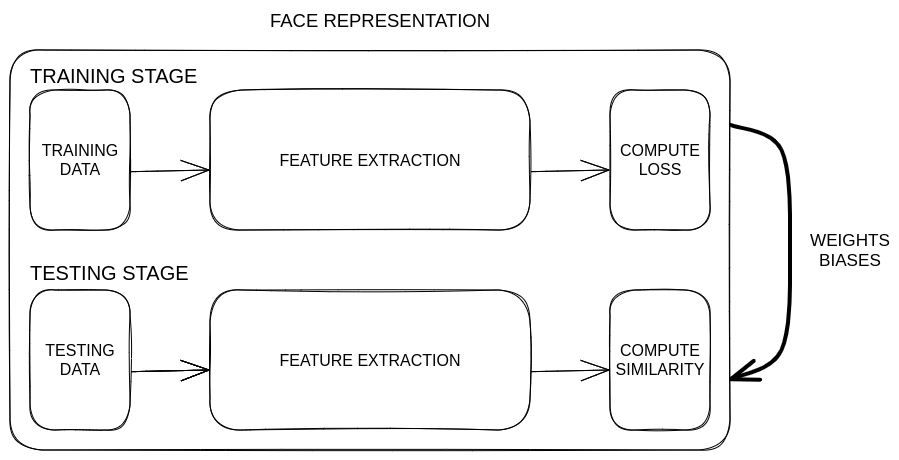
\includegraphics[scale=0.4]{frep_pipeline.png}
    \caption[Pipeline]{Face Representation pipeline, guided by the approach in~\autocite{wangDeepFaceRecognition2021}.}
    \label{fig:frep pipeline}
\end{figure}

\par As show in \reffig{fig:frep pipeline}, Face Representation is a two-step module composed of a training and testing stage. So as to be capable of performing face recognition, in either a verification or identification manner, a face representation system needs to learn robust, invariant and discriminative features that can distinguish identities~\autocite{ranjanDeepLearningUnderstanding2018}. 
\par To meet these requirements, the feature extractor must first be trained properly by taking data from previous stages and outputting a feature representation that's compared to the desired value using a loss function\footnote{Also referred to as a cost or objective function.~\autocite{lecunDeepLearning2015}}~\autocite{lecunDeepLearning2015, wangDeepFaceRecognition2021}. After that, everything is ready for the testing stage, where the face recognition \textit{per se} occurs by calculating a similarity score for the feature representation produced by the trained feature extractor, and dictating if the identity belongs to the same person (face verification) or if it matches any identity (face identification)~\autocite{ranjanDeepLearningUnderstanding2018}.



\subsection{Datasets: Training and Testing Data}
\par As been discussed throughout this dissertation, Deep Learning techniques can solve the problem of handling unconstrained scenarios, where there are variations in pose, illumination, occlusion, and so forth. To support this, in the past few years, datasets have been developed with this in mind so to be able to provide a large and diverse set of both training data, allowing for adequate regularization to unseen circumstances, and testing data that benchmarks the face recognition system in, as similar as possible, unconstrained real world scenarios~\autocite{duElementsEndtoendDeep2022}. 

\vspace{\baselineskip}
In the following pages, a mix of training datasets, of overall relevance and more geared towards the purpose of this dissertation, will be reviewed.

\subsubsection{\large Training Data}
\par When developing a deep face recognition system it's essential to keep in mind its necessity to adapt, and that's where the dataset used for training comes at play. Large training datasets are essential for face recognition~\autocite{parkhiDeepFaceRecognition2015}, but large-scale is not enough. There must be a balance between the depth (number of unique identities) and the breadth/width (number of images per identity)~\autocite{bansalDonTsCNNbased2017, caoVGGFace2DatasetRecognising2018}, and it will lead to different effects. 
\par On one hand, a training dataset that is deep will help the face recognition system to produce more discriminative feature representations, since it will have a great number of identities to learn from. On the other hand, a wider set will have more images per identity, therefore, variations in pose, expressions, illuminations, occlusions, background clutter, image quality, accessories, and so forth~\autocite{baeDigiFace1MMillionDigital2023} can be introduced and ultimately lead to feature representations more robust to them.

% \par Earlier works~\autocite{schroffFaceNetUnifiedEmbedding2015,sunDeepLearningFace2014,taigmanDeepFaceClosingGap2014} resourced private face datasets, but as time passed, more public datasets were released. 

\vspace{0.7\baselineskip}
\noindent\textbf{$\rightarrow$ CASIA-WebFace}~\autocite{yiLearningFaceRepresentation2014}, composed of 494,414 face images and 10,575 identities, was proposed as a novel dataset to overcome the problem of data dependence in face recognition and improve comparability across different methods. By training on the same dataset, methods can be better evaluated and compared.

\vspace{0.7\baselineskip}
\noindent\textbf{$\rightarrow$ VGGFace}~\autocite{parkhiDeepFaceRecognition2015} was published alongside a homonymous face recognition method and, once again, with the objective of combating the lack of available large scale public datasets. It contains 2,6 million images and 2,622 different identities and a curated version, where incorrect image labels were hand-removed by humans, has 800,000 images for the same amount of identities.

% Both datasets were released for training only purposes~\autocite{caoVGGFace2DatasetRecognising2018}.

% \vspace{0.7\baselineskip}
% \noindent\textbf{$\rightarrow$ CelebA} 2015

% \vspace{0.7\baselineskip}
% \noindent\textbf{$\rightarrow$ UMDFaces} 2015

\vspace{0.7\baselineskip}
\noindent\textbf{$\rightarrow$ MS-Celeb-1M}'s~\autocite{guoMSCeleb1MDatasetBenchmark2016} first intention was to provide a novel benchmark to identify celebrities that solves name ambiguities by linking a face with an entity key in a knowledge base. Second, it aimed at solving the gap in available large-scale datasets by providing a training set with, approximately, 10 million images and 100 thousand identities. Unfortunately, it is a dataset known for the presence of noisy labels. 

% That is mainly due to the size of the dataset, the automatic method of collecting and annotating the images, and also the fact that the noise is not removed on purpose (under the assumption that training with noisy data might be beneficial). 

\vspace{0.7\baselineskip}
\noindent\textbf{$\rightarrow$ MegaFace}~\autocite{nechLevelPlayingField2017} introduced a benchmark for million-scale face recognition and provided a public large-scale training dataset that integrated 4,753,320 faces over 672,057 identities. The main difference compared to the previously mentioned datasets is that MegaFace does not use celebrities as subjects, in contrast it leverages the photographs released by Flickr under the Creative Commons license. 

\vspace{0.7\baselineskip}
\noindent\textbf{$\rightarrow$ VGGFace2}~\autocite{caoVGGFace2DatasetRecognising2018} is another large-scale dataset, and its main goals are: 1) covering numerous identities, 2) reduce labeling noise through automatic and manual filtering and, finally, 3) represent more realistic unconstrained scenarios due to a novel dataset generation pipeline that gathers images with a broad range of poses, age, illumination and ethnicity. All in all, this resulted in a dataset comprised of 3,31 million faces of 9131 subjects.

\vspace{0.7\baselineskip}
\noindent\textbf{$\rightarrow$ UMDFaces-Videos}~\autocite{bansalDonTsCNNbased2017} is a video-based dataset composed of 22,075 videos of 3,107 subjects with 3,735,476 human annotated frames with great variation in image quality, pose, expressions and lightning. It was proposed during a study how the performance of a face verification models is impacted by the effects of: 1) the type of media used for training (only videos or still images vs a mixture of both), 2) the width and depth of a dataset, 3) the label's noise and 4) the alignment of the faces.


% training on a mixture of still images and videos boosts performance. There's a bias toward high quality images in still datasets due to the way of capturing the data (high quality cameras). Models trained only on still images perform poorly on frames extracted from videos, they're very challenging due to pose, expression and illumination variations. Models trained only on videos perform poorly on datasets composed of only still images.

% The introduction of noisy labels does not increase face verification performance, clean data always performs better. Although, the difference between a clean dataset and one with a low percentage of noise (less than 5\%) is very low.

\vspace{0.7\baselineskip}
\noindent\textbf{$\rightarrow$ Celeb-500k}~\autocite{caoCeleb500KLargeTraining2018} is another large-scale proposed with two issues in mind: the disparity in the scale of public datasets when compared with private ones, and determining the impact in performance from intra- and inter-class variations. That being so, Celeb-500k, consisting of 50 million images from 500 thousand persons, and Celeb-500k-2R, a cleaned version of the previous, comprised of 25 million aligned faces of 245 thousand identities, are released.

\vspace{0.7\baselineskip}
\noindent\textbf{$\rightarrow$ IMDb-Face}~\autocite{wangDevilFaceRecognition2018} proposes a new dataset with based on a manually cleaned revision of MS-Celeb-1M and MegaFace. The growing demand for large-scale datasets introduced a new variable to take into consideration: the time available to annotate the data. Datasets that are well-annotated and have an enormous amount of data are notably expensive and time-consuming to develop. Therefore, automatic measures to clean the data were used, so it's expected for a certain degree of noise to be introduced in a dataset. After selecting a subset from both the originals datasets, 2 million images were manually cleaned and resulted in 1,7 million images of 59 thousand celebrities.

\vspace{0.7\baselineskip}
\noindent\textbf{$\rightarrow$ MS1MV2}~\autocite{dengArcFaceAdditiveAngular} is another well know dataset. It was proposed in the ArcFace face recognition method's revision paper and consists of a semi-automatic refinement of the previously mentioned MS-Celeb-1M, resulting in 5,8 million images of 85 thousand identities.

\vspace{0.7\baselineskip}
\noindent\textbf{$\rightarrow$ RMFRD}~\autocite{wangMaskedFaceRecognition2020} is presented in the context of the need of using a mask, mandated by the COVID-19 pandemic, and that greatly reduces the effectiveness of conventional face recognition methods. Therefore, there was a need to improve their performance and for that a dataset that provides masked faces is needed. RMFRD pioneered this need by publishing a dataset consisting of 5 thousand masked and 90 thousand unmasked faces from 525 celebrities.

\vspace{0.7\baselineskip}
\noindent\textbf{$\rightarrow$ Glint360K}~\autocite{anPartialFCTraining2021} is a training set presented in the Partial FC method paper. It was generated by merging and cleaning the aforementioned Celeb-500K and MS1MV2 datasets, which resulted in 17 million images of 360 thousand individuals.

\vspace{0.7\baselineskip}
\noindent\textbf{$\rightarrow$ WebFace260M}~\autocite{zhuWebFace260MBenchmarkUnveiling2021} takes a giant leap in closing the gap between public available datasets and private ones. Partnered with a time-constrained face recognition protocol, the original paper presented an enormous 260 million faces and 4 million identities noisy dataset, an automatically cleaned, high quality training set with 42 million faces over 2 million identities (WebFace42M), and a smaller scale training dataset derived from the WebFace42M that has 10\% of its data (WebFace4M).
 % Traditional test datasets that focus on accuracy have been almost saturated
 % Interesting time-constrained face recognition protocol

\vspace{0.7\baselineskip}
\noindent\textbf{$\rightarrow$ DigiFace-1M}~\autocite{baeDigiFace1MMillionDigital2023} is a novel approach that revolutionizes the way of training face recognition models. It is a fully synthetic dataset that proposes mitigating three very relevant problems present in the majority of the conventional datasets: 1) ethical issues, 2) label noise and 3) data bias. The dataset is divided in two parts: part one contains 720 thousand images from 10 thousand identities and part two has 500 thousand images with 100 thousand identities, for a total of 1,22 million images and 110 thousand unique identities.

% Privacy violations, lack of informed consent and exploitation of distribution licenses or vague terms (such as "celebrities") to gather data are some of the criticisms that raised enough concerns that lead to revoking the distribution of several datasets. 

\begin{table}[!ht]
    \centering
    \resizebox{\textwidth}{!}{%
    \begin{tabular}{|l|c|c|c|c|c|c|c|}
    \hline
    \multicolumn{1}{|c|}{\textbf{Dataset}} & \textbf{Year} & \textbf{Availability} & \textbf{Images/videos} & \textbf{Depth} & \textbf{Avg. Breadth} & \textbf{Distribution} & \textbf{Description} \\ \hline
    CASIA-WebFace~\autocite{yiLearningFaceRepresentation2014}                         & 2014          & Discontinued          & 494,414/-              & 10,575         & 46.7                  & Public                & First public face recognition dataset.                 \\ \hline
    \textit{Facebook}~\autocite{taigmanWebscaleTrainingFace2015}                               & 2015          & -                     & 500M/-                 & 10M            & 50                    & Private               & \textit{Facebook}'s private dataset used to test different properties in face identification.                 \\ \hline
    \textit{Google}~\autocite{schroffFaceNetUnifiedEmbedding2015}                                 & 2015          & -                     & 200M/-                 & 8M             & 25                    & Private               & Private dataset used to train the FaceNet method.                 \\ \hline
    VGGFace~\autocite{parkhiDeepFaceRecognition2015}                                & 2015          & Discontinued          & 2,6M/-                 & 2,622          & 991.6                 & Public                & High width public dataset released alongside VGGFace method.                 \\ \hline
    MS-Celeb-1M~\autocite{guoMSCeleb1MDatasetBenchmark2016}                           & 2016          & Discontinued          & 10M/-                  & 100k           & 100                   & Public                & Large-scale celebrities dataset.                 \\ \hline
    MegaFace~\autocite{nechLevelPlayingField2017}                               & 2016          & Discontinued                  & 4,753,320/-            & 672,057        & 7.1                   & Public                & Non-celebrity dataset.                 \\ \hline
    VGGFace2~\autocite{caoVGGFace2DatasetRecognising2018}                               & 2017          & Discontinued                  & 3,31M/-                & 9131           & 362.5                 & Public                & High characteristics variation dataset.                 \\ \hline
    UMDFaces-Videos~\autocite{bansalDonTsCNNbased2017}                        & 2017          & Discontinued                  & -/22,075               & 3,107          & 7.1                   & Public                & Video-based dataset with great variations.                 \\ \hline
    Celeb-500k~\autocite{caoCeleb500KLargeTraining2018}                             & 2018          & Available                  & 50M/-                  & 500k           & 100                   & Public                & Noisy celebrities dataset.                 \\ \hline
    Celeb-500k-2R~\autocite{caoCeleb500KLargeTraining2018}                          & 2018          & Available                  & 25M/-                  & 245k           & 102                   & Public                & Cleaned version.                 \\ \hline
    IMDb-Face~\autocite{wangDevilFaceRecognition2018}                              & 2018          & Available                  & 1,7M/-                 & 59k            & 28.8                  & Public                & Manually cleaned revision of MS-Celeb-1M and MegaFace.                 \\ \hline
    MS1MV2~\autocite{dengArcFaceAdditiveAngular}                                 & 2019          & Available                  & 5,8M/-                 & 85k            & 68.2                  & Public                & Semi-automatic cleaned version of MS-Celeb-1M.                 \\ \hline
    RMFRD~\autocite{wangMaskedFaceRecognition2020}                                 & 2020          & Available                  & 95k/-                  & 525            & 180.9                 & Public                & Dataset of masked and unmasked celebrities.                 \\ \hline
    Glint360k~\autocite{anPartialFCTraining2021}                              & 2021          & Available                  & 17M/-                  & 360k           & 47.2                  & Public                & Cleaned version of the Celeb-500k AND MS1MV2 datasets.                \\ \hline
    WebFace260M~\autocite{zhuWebFace260MBenchmarkUnveiling2021}                            & 2021          & Available                  & 260M/-                 & 4M             & 65                    & Public                & Largest publicly available dataset of celebrities faces (noisy).                 \\ \hline
    WebFace42M~\autocite{zhuWebFace260MBenchmarkUnveiling2021}                             & 2021          & Available                  & 42M/-                  & 2M             & 21                    & Public                & Cleaned and smaller version.                 \\ \hline
    WebFace4M~\autocite{zhuWebFace260MBenchmarkUnveiling2021}                              & 2021          & Available                  & 4,2M/-                 & 200k           & 21                    & Public                & Smaller version.                 \\ \hline
    DigiFace-1M~\autocite{baeDigiFace1MMillionDigital2023}                            & 2022          & Available                  & 1,22M/-                & 110k           & 11.1                  & Public                & Large-scale, fully synthetic dataset.                 \\ \hline
    \end{tabular}%
    }
    \caption{Comparison table of the previously described training datasets.}
    \label{tab:training data}
\end{table}
\newpage
\subsubsection{\large Testing Data}

\par After the training is completed the performance of the system needs to be evaluated on different challenges to properly access if it scales (or generalizes or applies or performs in) to real-world scenarios. A test dataset can be chosen for specific hurdles, for instance, cross-pose, cross-age, racial variations, quality assessment, and so forth~\autocite{duElementsEndtoendDeep2022}.


\vspace{0.7\baselineskip}
\noindent\textbf{$\rightarrow$ LFW}~\autocite{huangLabeledFacesWild} is the most well-known face verification dataset. It was first released in 2007 as a way of evaluating the performance of face recognition methods, in a verification or pair matching manner, under unconstrained scenarios. LFW divides the dataset in 2 views. View 1 is designed for development, and in the training set contains 1100 pairs of mismatched images and 1100 pairs of matched ones, while the test set has 500 pairs of matched and 500 pairs of unmatched faces. View 2 is intended for performance reporting and splits the data over 10 separate sets, to facilitate 10-fold cross validation, where each one has 300 positive pairs (same identity) and 300 negative pairs (different person), resulting in 6000 pairs. Overall, the dataset has 13,233 face images and 5749 identities (only 1680 persons have two or more images).

\vspace{0.7\baselineskip}
\noindent\textbf{$\rightarrow$ YTF}~\autocite{wolfFaceRecognitionUnconstrained2011} is a video-based benchmark that leverages the greater amount of information provided by a video in comparison to still images. By collecting videos from \textit{Youtube} there isn't an opportunity to control the conditions, hence the footage will support a wider range of characteristic's variation, namely lighting conditions, difficult poses, motion blur, compression artifacts, etc. This resulted in 3425 videos from 1595 identities and a benchmark protocol inspired in the LFW. To evaluate performance, a pair-matching test is designed. From the database, 5000 video pairs are collected, where half are matches and the other half are not, to be divided to allow 10-fold cross validation.

\vspace{0.7\baselineskip}
\noindent\textbf{$\rightarrow$ IJB-A}~\autocite{klarePushingFrontiersUnconstrained2015} aims at straying further from the saturation in recognition benchmarks by proposing more challenging benchmarks (specifically by including wider geographic distribution and full pose variation) for both verification and identification. It consists of a mix of 5712 images and 2085 videos from 500 individuals, with manual bounding boxes, facial landmarks and, most importantly, labels. IJB-A supports two protocols: search (face identification) and compare (face verification). For both the protocols, the specifications are the same, i.e., ten random training and testing splits are generated using all 500 identities then used to perform sample bootstrapping (instead of cross validation) in order to enhance the number of testing subjects. For each split, 333 subjects are randomly distributed in the training set and the remainder 167 are placed in the testing set.

\vspace{0.7\baselineskip}
\noindent\textbf{$\rightarrow$ CFP}~\autocite{senguptaFrontalProfileFace2016} studies the effect of extreme pose variations, such as a profile view of a face, in face verification. During collection gender and profession balance, as well as racial diversity, were considered. A number of frontal and profile view images was also set as 10 and 4, respectively. Therefore, after cleaning the initial data, it resulted in 7000 images from 500 subjects. The experimental protocol divided the 500 identities over 10 splits (facilitating 10-fold cross validation) and randomly generated 7 matched pairs and 7 unmatched pairs per identity, resulting in a total of 7000 pairs of faces.

\vspace{0.7\baselineskip}
\noindent\textbf{$\rightarrow$ MegaFace2}~\autocite{nechLevelPlayingField2017} has already been mentioned in the Training Data section, with exception to detailing the benchmarking protocol. The MegaFace2 is used to train the model that will be tested in 3 datasets: a one million Flickr distraction set, FaceScrub~\autocite{ngDatadrivenApproachCleaning2014} and FG-Net. The first dataset is intended to supply the model with identities that are not to be found (hence being called a distraction set), while the last two contain the known identities to be tested.

\vspace{0.7\baselineskip}
\noindent\textbf{$\rightarrow$ CPLFW}~\autocite{zhengCrossPoseLFWDatabase} is another dataset that tackles the overly optimistic accuracy saturation in classic benchmarks, such as the previously mentioned LFW. To this end, evaluating performance for cross-pose faces of LFW subjects is the matter of study. It contains the same number of 13,233 images of 5749 identities like LFW and the benchmark protocol performance is the LFW \textit{View 2} with some differences: 1) negative pairs are from people of the same race and gender, 2) class imbalance and limited positive pair's diversity is resolved by assuring that each identity has at least 2 images.

\vspace{0.7\baselineskip}
\noindent\textbf{$\rightarrow$ CALFW}~\autocite{zhengCrossAgeLFWDatabase2017} has the same principles as CPLFW but applied to the age of the subjects (including the negative pairs selection and the class imbalance problem).

\vspace{0.7\baselineskip}
\noindent\textbf{$\rightarrow$ Age-DB}~\autocite{moschoglouAgeDBFirstManually2017}, similarly to CALFW, is a dataset that considers the subject's age. It distances itself from other databases by solving the noisy labelling, induced by automatic or semi-automatic methods, by doing so manually. Age-DB has 16,488 images and 568 subjects used in 4 evaluation protocols, similar to LFW's \textit{View 2}, where the main difference between them is the age difference between pairs (5, 10, 20 and 30 years).

\vspace{0.7\baselineskip}
\noindent\textbf{$\rightarrow$ IJB-B}~\autocite{whitelamIARPAJanusBenchmarkB2017} builds upon IJB-A and proposes solving flaws that were verified in the previous dataset. First, the improved IJB-B dataset is larger, consisting of 21,798 images and 7,011 videos from 1,845 subjects, with a more uniform racial distribution. Second, the protocols are upgraded due to a greater number of possible comparisons between images and possible identities.

\vspace{0.7\baselineskip}
\noindent\textbf{$\rightarrow$ TinyFace}~\autocite{chengLowResolutionFaceRecognition2019} was presented to fill in the gap of low-resolution face recognition benchmarks with genuine images and not downsampled ones. It is designed for face identification, and is composed of 15,975 labelled images and 153,428 distractors, totalling 169,403 low resolution images, from 5,139 identities. The evaluation protocol is similar to the one used by MegaFace: 1) half of the identities are randomly sampled by the probe set and the other half by the gallery set, and 2) the distractor images are added to the gallery incorporating further complexity to the identification process.

\vspace{0.7\baselineskip}
\noindent\textbf{$\rightarrow$ IJB-C}~\autocite{mazeIARPAJanusBenchmark2018} adds 1661 new identities to IJB-B and new end-to-end protocols (to evaluate face detection, identification, verification, clustering) in order to better mimic real-world unconstrained recognition. They have increased diversity, both in geographic location and profession, and occlusion scenarios. IJB-C has 31,334 images and 11,779 videos from 3531 subjects.

\vspace{0.7\baselineskip}
\noindent\textbf{$\rightarrow$ IJB-S}~\autocite{kalkaIJBIARPAJanus2018} is a manually annotated benchmark constructed by collecting images and surveillance videos that presents a challenging face recognition problem. It is a dataset with several challenging variations, namely, full pose, resolution, presence of motion blur and visual artifacts. The aforesaid are tested during 6 different face detection and identification protocols. IJB-S consists of 350 surveillance videos, 202 enrollment videos and 5656 images. 

\vspace{0.7\baselineskip}
\noindent\textbf{$\rightarrow$ RFW}~\autocite{wangRacialFacesWild2019} is a proposed benchmark dataset to evaluate the racial bias of face verification solutions. It is divided in 4 subsets regarding the race of the subjects, where each contains, approximately, 10 thousand images and 3 thousand identities, totaling 40,607 images from 11,429 subjects. The evaluation protocol is the same as the LFW one, but the negative pairs were mined to be difficult and avoid easily saturated performance.

\vspace{0.7\baselineskip}
\noindent\textbf{$\rightarrow$ QMUL-SurvFace}~\autocite{chengSurveillanceFaceRecognition2018} is a dataset introduced as a benchmark in the \textit{Surveillance Face recognition Challenge} for face recognition in a surveillance context, and it contains both face verification and identification protocols. By data-mining 17 public person re-identification datasets, it achieves 463,507 facial images of 15,573 identities collected in uncooperative surveillance scenarios. Consequently, it presents a high variance in resolution, motion blur, pose, occlusion, illumination and background clutter.

\vspace{0.7\baselineskip}
\noindent\textbf{$\rightarrow$ MDMFR}~\autocite{ullahNovelDeepMaskNetModel2022} is brought about in light of the COVID-19 impact, where wearing a mask became mandatory and rendered unusable the traditional face recognition methods. Therefore, in conjunction with DeepMaskNet, MDMFR was released. It is a large-scale benchmark dataset designed to evaluate the performance of both masked face recognition and masked face detection algorithms. The recognition protocol contains 2896 images from 226 identities, intended to benchmark masked face recognition models.

\vspace{0.7\baselineskip}
\noindent\textbf{$\rightarrow$ XQLFW}~\autocite{knocheCrossQualityLFWDatabase2021} revisits the LFW and modifies it to better evaluate cross-resolution face recognition problems. The evaluation protocol, number of images and identities remains the same (13,233 and 5749, respectively), but the negative pairs are sampled in the same manner as CPLFW~\autocite{zhengCrossPoseLFWDatabase} and CALFW~\autocite{zhengCrossAgeLFWDatabase2017}.

\vspace{0.7\baselineskip}
\noindent\textbf{$\rightarrow$ CAFR}~\autocite{zhaoAgeInvariantFaceRecognition2022} was introduced in 2022, in the revised paper of the AIM (Age-Invariant Model) as a large-scale benchmark dataset to advance the development of face recognition models invariant to age. It consists of 1,446,500 images from 25,000 subjects and spans a range of ages from 1 to 99 years old. The evaluation protocol divides the data in 10 splits of 2500 pair-wise disjoint subjects, where each one has associated to it 5 matched pairs and 5 unmatched, resulting in a total of 25,000 pairs per split.

\vspace{0.7\baselineskip}
\noindent\textbf{$\rightarrow$ FaVCI2D}~\autocite{popescuFaceVerificationChallenging2022} is face verification benchmark dataset that proposes to address three relevant flaws : 1) the pairs selected are not challenging enough,  2) the demographics of other datasets are not representative enough of the real world diversity and 3) legal and ethical questions concerning the data used. It is composed of 64,879 images and 52,411 unique identities, where 12,468 are used to create genuine matched identity pairs with balanced gender and geographic distribution.

\begin{table}[!ht]
    \centering
    \resizebox{\textwidth}{!}{%
    \begin{tabular}{|l|c|c|c|c|c|c|c|}
    \hline
    \multicolumn{1}{|c|}{\textbf{Dataset}} & \textbf{Year} & \textbf{Availability} & \textbf{Images/videos} & \textbf{Depth} & \textbf{Avg. Breadth} & \textbf{Distribution} & \textbf{Description} \\ \hline
    LFW~\autocite{huangLabeledFacesWild}                                    & 2007          & Discontinued          & 13,233/-              & 5,749         & 2.3                  & Public                & The most well known face verification public dataset.                 \\ \hline
    YTF~\autocite{wolfFaceRecognitionUnconstrained2011}                                    & 2011          & Available                     & -/3,425                 & 1595            & 2.1                    & Public               & Face verification video dataset inspired on the LFW                 \\ \hline
    IJB-A~\autocite{klarePushingFrontiersUnconstrained2015}                                  & 2015          & Discontinued                     & 5,712/2,085                 & 500             & 11.4/4.2                    & Public               & Benchmark that aims at straying from accuracy saturation by proposing a more challenging dataset.                 \\ \hline
    CFP~\autocite{senguptaFrontalProfileFace2016}                                 & 2016          & Discontinued          & 7,000/-                 & 500          & 14                 & Public                & Studies the effect of extreme pose variations on face verification.                 \\ \hline
    \red{MegaFace2*}~\autocite{nechLevelPlayingField2017}                              & 2016          & Discontinued          & 10M/-                  & 100k           & 100                   & Public                & temp                 \\ \hline
    CPLFW~\autocite{zhengCrossPoseLFWDatabase}                                  & 2017          & Available                  & 13,233/-            & 5,749        & 2.3                   & Public                & Variation of the LFW for different poses with refined verification pairs.                 \\ \hline
    CALFW~\autocite{zhengCrossAgeLFWDatabase2017}                                  & 2017          & Available                  & 13,233/-                & 5,749           & 2.3                 & Public                & Same principles of CPLFW but applied to age related tests.                 \\ \hline
    AgeDB~\autocite{moschoglouAgeDBFirstManually2017}                                  & 2017          & Available                  & 16,488/-               & 568          & 29.0                   & Public                & Similar to CALFW but promotes noise free labelling by doing it manually.                 \\ \hline
    IJB-B~\autocite{whitelamIARPAJanusBenchmarkB2017}                                 & 2017          & Discontinued                  & 21,798/7,011                  & 1,845           & 11.8/3.8                   & Public                & Improvement over the IJB-B dataset (more data and more possible pairs).                 \\ \hline
    TinyFace~\autocite{chengLowResolutionFaceRecognition2019}                               & 2018          & Available                  & 15,975 (153,428)/-                  & 5,139           & 3.1                   & Public                & Genuine low resolution face recognition benchmark.                 \\ \hline
    IJB-C~\autocite{mazeIARPAJanusBenchmark2018}                                  & 2018          & Discontinued                  & 31,334/11,779                 & 3,531            & 8.9/3.3                  & Public                & IJB-B refinement (more protocols and increased individuals diversity).                 \\ \hline
    IJB-S~\autocite{kalkaIJBIARPAJanus2018}                                  & 2018          & Discontinued                  & 5,656/350 (202)                 & 202            & 28/2.7                  & Public                & Very challenging manually annotated benchmark.                 \\ \hline
    RFW~\autocite{wangRacialFacesWild2019}                                    & 2018 & Available                  & 40,607/-                  & 11,429            & 3.5                 & Public                & Benchmarks the racial bias of face verification methods.                 \\ \hline          
    QMUL-SurvFace~\autocite{chengSurveillanceFaceRecognition2018}                          & 2018          & Available                  & 463,507/-                  & 15,573            & 29.8                 & Public                & Dataset colected in uncooperative surveillance scenarios, presenting high variance of characteristics.                  \\ \hline
    MDMFR~\autocite{ullahNovelDeepMaskNetModel2022}                                  & 2021          & Available                  & 2,896/-                  & 226            & 12.8                 & Public                & Large scale dataset for masked face recognition.                 \\ \hline
    XQLFW~\autocite{knocheCrossQualityLFWDatabase2021}                                  & 2021          & Available                  & 13,233/-                  & 5,749           & 2.3                  & Public                & LFW variation to study the effect of resolution on face verification.                 \\ \hline
    CAFR~\autocite{zhaoAgeInvariantFaceRecognition2022}                                   & 2022          & Available                  & 1,446,500/-                  & 25,000            & 57.9                 & Public                & Large scale dataset to study the impact of individual's age.                 \\ \hline
    FaVCI2D~\autocite{popescuFaceVerificationChallenging2022}                                & 2022          & Available                  & 64,879/-                 & 52,411             & 1.2                    & Public                & Face verification dataset that addresses unchallenging pairs, demographic bias and ethical concerns.                 \\ \hline
    \end{tabular}%
    }
    \caption{Comparison table of the previously described test datasets.}
    \label{tab:test data}
\end{table}

\vspace{\baselineskip}
\par Although some of the previously referenced datasets do have a benchmarking component and are described as such, they can also be generally employed to train algorithms. When it is desired to fine-tune\footnote{An approach to transfer learning (producing a new model by using a pre-trained as a starting point)~\autocite{zhuangComprehensiveSurveyTransfer2020}. More details on this topic in the section \hyperref[transf learning]{Transfer Learning}.} a model for a specific challenge that, usually,  can be better achieved by employing a "benchmark" dataset that was purposefully developed to evaluate a model's performance on that exact challenge. 

\vspace{\baselineskip}
\centerline{
    \noindent
    \fbox{
        \begin{minipage}{0.95\textwidth}
            \centering
            \noindent A common denominator throughout the machine learning domain, and more specifically deep learning, is a general difficulty in separating concepts with a single line. This is a non-linear science in its nature.
        \end{minipage}
    }
}

\vspace{\baselineskip}
\subsection{Feature Extractor}
A feature extractor is present in both the training and testing stage of the Face Representation process, and comprehends a fundamental part of it, as it is what allows the visual data to be processed and transformed to be evaluated, by transforming the input into low dimensional representations~\autocite{lecunGradientBasedLearningApplied1998}. It is also what distinguishes a Conventional Machine Learning approach from a Deep Learning one.  
\par Being that the following methods are all based in deep learning, therefore, the \textit{modus operandi} abides by the same principles and can be outlined as follows: 1) the feature extractor is a deep neural network, more specifically a Convolutional Neural Network (CNN), that is trained with a loss function, 2) the trained feature extractor contains prior knowledge and is applied on unseen test data and 3) the results are used to compute 1:N similarity (face identification - "who is this person?") or 1:1 similarity (face verification - "are these persons the same?").
\par Over the years, the architecture of CNNs evolved and became of great importance to all image related tasks. Other than the already mentioned revolutionary AlexNet~\autocite{krizhevskyImageNetClassificationDeep2012}, there are other designs that significantly contributed to breakthroughs and broken benchmark records. There can be general architectures, suchlike VGGNet~\autocite{simonyanVERYDEEPCONVOLUTIONAL2015}, GoogLeNet~\autocite{szegedyGoingDeeperConvolutions2014}, ResNet~\autocite{heDeepResidualLearning2016}, iResNet~\autocite{dutaImprovedResidualNetworks2021}, or specialized architectures. For example, lightweight face recognition implementations such as MobileFaceNet~\autocite{chenMobileFaceNetsEfficientCNNs2018}, VarGFaceNet~\autocite{yanVarGFaceNetEfficientVariable2019}, MixFaceNet~\autocite{boutrosMixFaceNetsExtremelyEfficient2021} and ConvFaceNeXt~\autocite{hooConvFaceNeXtLightweightNetworks2022}.

\newpage
% \vspace{0.7\baselineskip}
\noindent\textbf{$\rightarrow$ VGGNet}~\autocite{simonyanVERYDEEPCONVOLUTIONAL2015} took inspiration from AlexNet and improved its accuracy in image classification by studying the effect of the network's depth. It accomplished that by substituting the 11x11 convolution kernel with stride 4 for a stack of very small 3x3 receptive field with stride 1. The final best performing model was 19 layers deep (16 convolutional and 3 fully-connected) and had 144 million parameters.

\begin{figure}[!h]
    \centering
    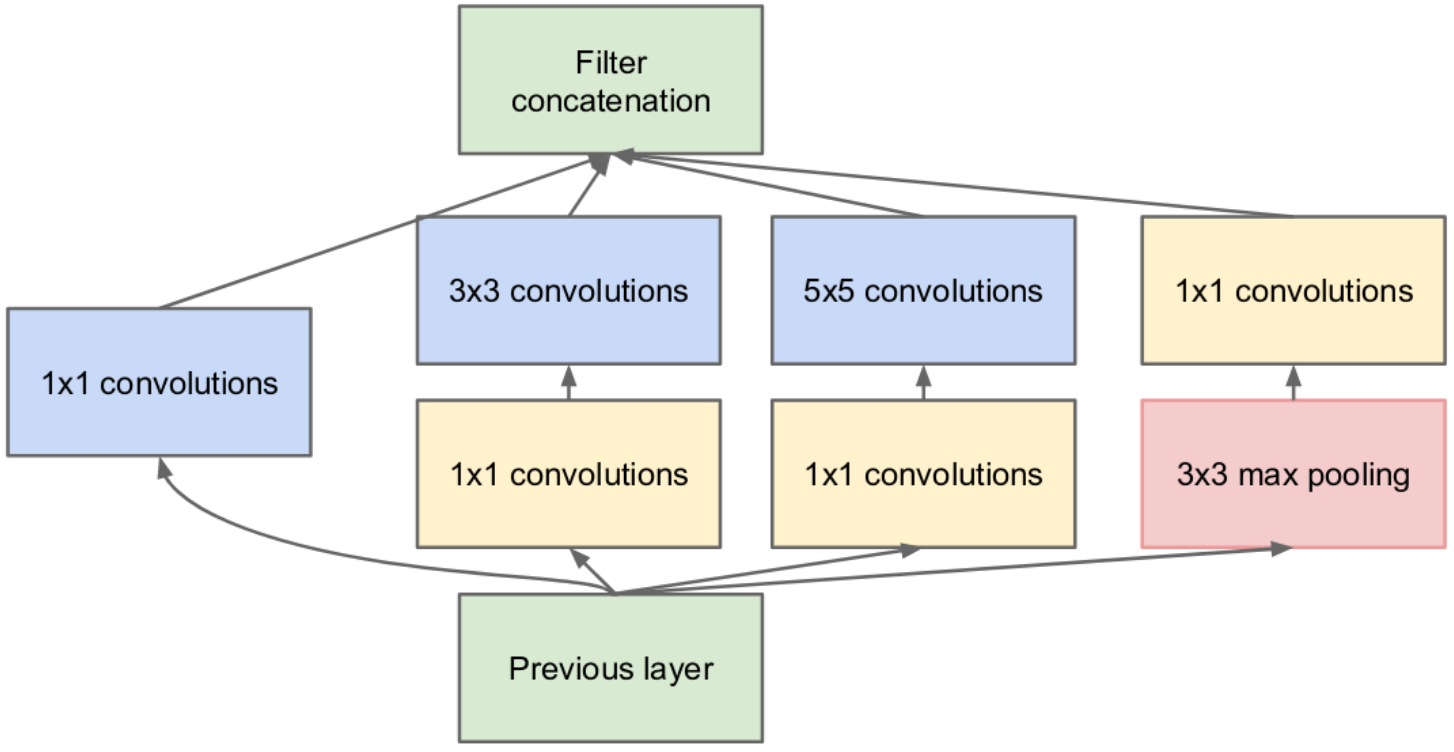
\includegraphics[scale=0.16]{inception.png}
    \caption{GoogLeNet architecture}
    \label{fig:inception}
\end{figure}

\vspace{0.7\baselineskip}
\noindent\textbf{$\rightarrow$ GoogLeNet}~\autocite{szegedyGoingDeeperConvolutions2014}, also known as Inception-V1, aimed at reducing the computational cost associated with training and employing a network, while retaining highly accurate results. That was accomplished by introducing an inception black, consisting of multi-scale convolutional layers with small blocks of different sized kernels (1x1, 3x3 and 5x5). By doing so, it allowed the network to capture information at different scales and increasing both the width and the depth without compromising computational costs. Additionally, sparse connectivity (not all feature maps are shared with the forward layers), replacing the last fully connected layer with a global averaging pooling one and adding a dimension lowering bottleneck layer of 1x1 convolution before employing large kernels, helped to achieve a significantly lower number of 4 million parameters (12x fewer than the revolutionary AlexNet and 36x less than VGGNet). This resulted in its victory on the 2014 ImageNet Large Scale Visual Recognition Challenge (ILSVRC) with a 22 layers deep model.

\begin{figure}[!h]
    \centering
    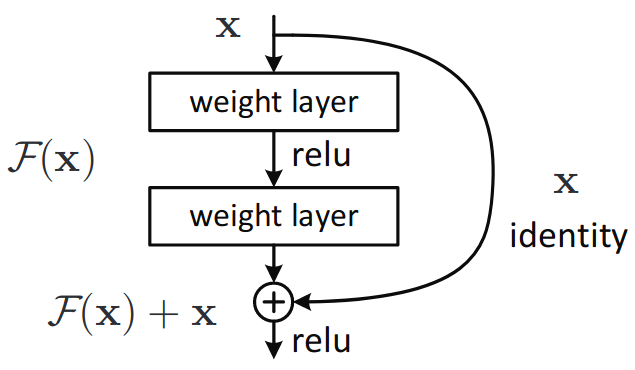
\includegraphics[scale=0.3]{residual.png}
    \caption{ResNet's residual block}
    \label{fig:residual}
\end{figure}

\vspace{0.7\baselineskip}
\label{sec:resnet}
\noindent\textbf{$\rightarrow$ ResNet}~\autocite{heDeepResidualLearning2016} is one of the most resourced architecture of feature extractors when applied to face recognition. Its main objective is to efficiently train deeper neural networks that are remarkably more difficult to do so. By reformulating the layers as residual learning functions, it supports deeper architectures while being easier to optimize and, at the same time, producing more accurate results. It also solves the accuracy degradation and the vanishing gradient problems verified when the depth of the network is increased. The main contribution is the introduction of the residual block \reffig{fig:residual}. It consists of convolutional layers, followed by element-wise addition between the output and the input of the block. This addition performs an identity mapping by creating a direct "shortcut connection" that skips the input directly to the output, allowing the network to learn the difference between the input and the output, i.e., the residual. Enabling the flow of information from earlier layers directly to later layers, facilitates the gradient flow during training and makes it easier for the network to learn. Depending on the depth, there are different variations of the ResNet architecture: ResNet-18 (11.7 million parameters), ResNet-34 (21.8 million parameters), ResNet-50 (25.6 million parameters), ResNet-101(44.6 million parameters), ResNet-152 (60.2 million parameters). The ResNet-152 won the 2015 ImageNet Large Scale Visual Recognition Challenge (ILSVRC), and it was 20 and 8 times deeper than AlexNet and VGGNet, respectively, while being less computational demanding.

\newpage
% \vspace{0.7\baselineskip}
\noindent\textbf{$\rightarrow$ iResNet}~\autocite{dutaImprovedResidualNetworks2021} further improves the ResNet architecture. It proposes: 1) a separation of the network into stages, providing a better path of information flow through the network's layers, 2) an introduction of an enhanced version of the residual learning block with 4 times more spatial channels that focus on the spatial convolution, and 3) an introduction of an improved projection shortcut (used when the dimensions of the previous blocks doesn't match the ones of the next) that includes an additional 3x3 max pooling. A major advantage is that all the improvements above do not increase the original model's parameters and, consequently, overall complexity.

\vspace{0.7\baselineskip}
\phantomsection\label{mobilefacenet}
\noindent\textbf{$\rightarrow$ MobileFaceNet}~\autocite{chenMobileFaceNetsEfficientCNNs2018} is a set of face verification CNN models designed to perform in real time and with high accuracy on mobile and embedded devices. It is built upon the inverted residual bottlenecks proposed in the general architecture lightweight CNN MobileNetV2~\autocite{sandlerMobileNetV2InvertedResiduals2019} that have the purpose of reducing the number of parameters of the network. The general residual bottleneck block~\autocite{heDeepResidualLearning2016} is composed of an input, followed by bottlenecks to reduce dimension and finished with an expansion to restore it, and the shortcut connects the high dimension layers. On the other hand, in the inverted residual architecture, it is considered that the information is stored in the bottleneck layers and the expansion is a mere implementation detail, therefore, a shortcut is placed directly between the bottlenecks. To solve the accuracy problem of face recognition CNNs that have a global average pooling layer, MobileFaceNets replaces it by a global depthwise convolution layer with kernel of size 7x7x1280 followed by a 1x1 convolution as the feature output layer. The primary MobileFaceNet architecture has 0.99 million parameters, but there is also the MobileFaceNet-M (the final 1x1 convolution is removed) and the MobileFaceNet-S (the 1x1 linear convolution before the global depthwise convolution is also removed).

\newpage
% \vspace{0.7\baselineskip}
\noindent\textbf{$\rightarrow$ VarGFaceNet}~\autocite{yanVarGFaceNetEfficientVariable2019} is a lightweight face recognition CNN implmentation based on the VarGNet architecture~\autocite{zhangVarGNetVariableGroup2020} that introduced a variable group convolution to solve unbalance of computational intensity due to hardware and compilers optimization. VarGFaceNet will use the normal and downsampling blocks from the VarGNet CNN, but will add a Squeeze and Excitation (SE) block~\autocite{huSqueezeandExcitationNetworks2019} and replace the usual ReLU activation function by the PReLU~\autocite{heDelvingDeepRectifiers2015} one, since it is better for face recognition tasks. Other than that, the head setting is also changed without losing discriminative ability. The network is started with a 3x3 convolution with stride 1 that preserves the input size, instead of the downsampling 3x3 one with stride 2 from VarGNet. Finally, the embedding setting is also modified by performing variable group convolution and pointwise convolution to shrink the feature map to a 512-dimensional feature vector that's fed to the fully connected layer. However, this shrinking can lead to loss of information, accordingly, to counter that, the number of channels of the feature map is expanded after the last convolution layer, and only then the variable group convolution is performed, decreasing the number of parameters and computation overhead while not degrading the information. In conclusion, the VarGFaceNet network is capable of performing accurate face recognition while maintaining a lower amount of 5 million parameters.

\vspace{0.7\baselineskip}
\noindent\textbf{$\rightarrow$ MixFaceNet}~\autocite{boutrosMixFaceNetsExtremelyEfficient2021} is a lightweight implementation of MixNet~\autocite{tanMixConvMixedDepthwise} tailored for face verification. MixNet introduced Mixed Depthwise Convolution Kernels (MixConv) that extends the theory behind depthwise convolution, but employs multiple kernel sizes in a single convolution, promoting the capturing of different patterns from distinct resolutions while reducing the number of parameters needed. The main differences proposed by the MixFaceNet design compared to MixNet resides in the head and embedding settings. For the network head set-up, fast downsampling in the first convolution layer with a 3x3 kernel and stride of 2, and PReLU~\autocite{heDelvingDeepRectifiers2015} activation function are used. Regarding the embedding settings, the global average pooling layer used by the MixNet architecture is replaced by a global depthwise convolution, in the same manner as the previously described \hyperref[mobilefacenet]{MobileFaceNet}. Additionally, a shuffle operation is also introduced to the MixConv block. All in all, 3 networks were proposed, MixFaceNet-XS, MixFaceNet-S and MixFaceNet-M, that would be added the prefix "Shuffle" if trained using the aforesaid shuffle operation. Both MixFaceNet-S and ShuffleMixFaceNet-S have 3.07 million parameters.

\vspace{0.7\baselineskip}
\noindent\textbf{$\rightarrow$ ConvFaceNeXt}~\autocite{hooConvFaceNeXtLightweightNetworks2022} is a family of lightweight face recognition models, based on the ConvNeXt and MobileFaceNets architectures. The original ConvNeXt block is modified to better adapt to face recognition tasks and optimized to reduce the number of parameters. Accordingly, the Enhanced ConvNext (ECN) block is designed by adopting a smaller 3x3 kernel during the depthwise convolution, instead of the original 7x7 one. Adopting the principles studied in the MobileFaceNets implementation, rather than the usual layer of normalization and GeLU in the ConvNeXt model, batch normalization and PReLU~\autocite{heDelvingDeepRectifiers2015} are employed. The overall ConvFaceNeXt architecture has 3 main components: the stem partition, the bottleneck partition and the embedding partition. The stem partition is similar to the previously referred "head settings" and is responsible for downsampling the data, and it can be deployed in two settings. The first setting is called patchify head (PH) and utilizes 2x2 convolutions with a stride of two, and the second setting is the typical head (TH) that maintains the stride and changes the kernel size to 3x3. The bottleneck partition is responsible for reducing the number of floating point operations (FLOPs)\footnote{Not to be confused with FLOPS (Floating point operations per second), a unit of computation speed}. Finally, the embedding partition, which is the stage where the face representation (or embedding) is obtained, and instead of average pooling and fully connected layers, once again, global depthwise convolution is engaged. Fine-tuning to the three partitions resulted in 4 different networks: ConvFaceNeXt\_PS and ConvFaceNeXt\_TS, both with 0.96 million parameters, as well as ConvFaceNeXt\_PE and ConvFaceNeXt\_TE, both with 1.05 million parameters.

\subsection{Loss}

\begin{figure}[!h]
    \centering
    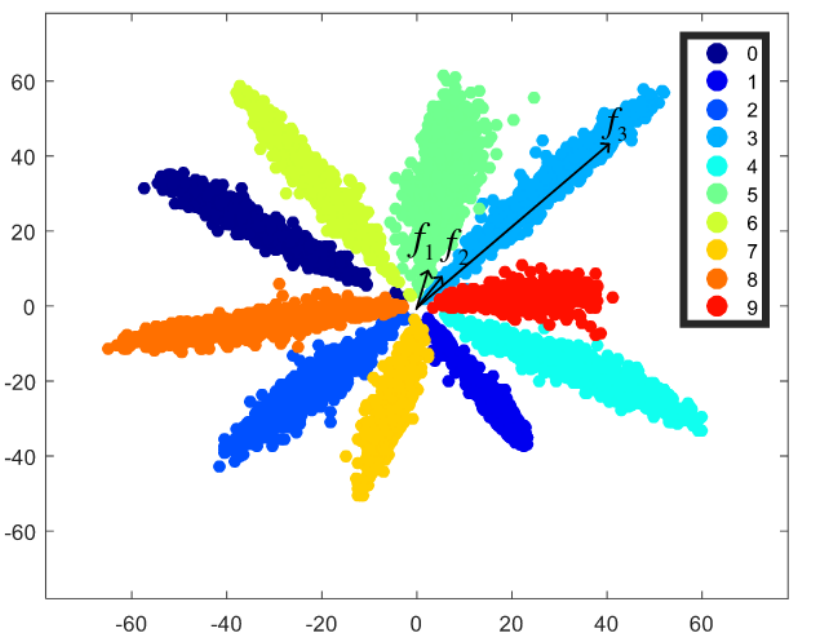
\includegraphics[scale=0.3]{compactness.png}
    \caption{Intra- and Inter-class challenge \autocite{wangNormFaceL2Hypersphere2017}. Eventhough features $f_2$ and $f_3$ belong to the same class, the euclidean distance between $f_1$ and $f_2$ is much smaller, proving the ineffectiness of the softmax loss regarding inter-class compactness and inter-class separateness.}
    \label{fig:compactness}
\end{figure}

The initial face recognition proposals inherited principles from successful object classification implementations, henceforth, the most common loss function utilized was the well-known softmax loss. Unfortunately, it soon proved to be inefficient for face recognition applications since intra-variations (age gap between pictures of the same identity, for example) can be larger than inter-ones \reffig{fig:compactness}. Thus, the investigation interest shifted towards developing loss functions that had a better generalization ability and promoted more separable (to distinguish between an identity) and discriminative (to distinguish between identities) features~\autocite{wangDeepFaceRecognition2021}.
\par Face recognition can be achieved using either metric learning loss functions that learn a feature embedding to compute similarity or softmax-based loss functions that treat the problem as a classification task. Some works merge the two concepts.

\subsubsection{Classification-based loss functions}
Classification-based loss functions, derived from the general object classification task, aim at learn an N-way classification of all the classes, where each class relates to an identity composed of several faces~\autocite{duElementsEndtoendDeep2022}.
\par Because the methods are classification-based, the pioneers such as DeepFace or DeepID~\autocite{sunDeepLearningFace2014a}, utilized the most widely implemented loss function for classification, i.e. the softmax loss. It consists of a fully connected layer, the softmax function and cross-entropy loss, and can be formulated as follows:
\begin{equation}
\mathcal{L} = -\frac{1}{N}\sum_{i=1}^{N}\log{\frac{e^{W_{y_i}^{T}x_i+b_{y_i}}}{\sum_{j=1}^{c}e^{W_{j}^{T}x_i+b_{j}}}},
\end{equation}

\noindent where $N$ is the number of images, $c$ is the number of identities, $y_i$ is the $x_i$'s ground-truth label, $W_{y_i}$ is the ground-truth weight from $x_i$ in the fully connected layer and $b_j$ is a bias term. The term inside the logarithm represents the probability on the ground-truth class and the training objective is to maximize this probability.

\vspace{\baselineskip}
\par Taking the aforementioned principles and the drawbacks of lackluster generalization, and separable/discriminative abilities, the following loss functions proposed improving the softmax loss to better serve face recognition tasks.

\vspace{0.7\baselineskip}
\noindent\textbf{$\rightarrow$ NormFace (2017)}~\autocite{wangNormFaceL2Hypersphere2017} improves the classic softmax loss by studying the effect of $L_2$ normalization to the features and weights during the training stage. Because introducing this constraint resulted in the network not converging, a scale factor is also adopted that resizes the cosine similarity's scale between features and weights. This normalized softmax loss function can de reformulated as
\begin{equation}
\mathcal{L}_{norm} = -\frac{1}{N}\sum_{i=1}^{N}\log{\frac{e^{s \cos{(\theta_{y_i})}}}{e^{s \cos{(\theta_{y_i})}}+\sum_{j=1, j\neq y_i}^{c}s \cos{(\theta_{j})}}},
\end{equation}

\noindent where $s$ is the scale parameter and $\cos{(\theta_j)}$ results from the inner product between the $L_2$ normalized  weights $W_j$ and features $x_i$, i.e., $\cos{(\theta_j)}=\frac{\langle x_i, W_j\rangle}{\|W_j\|_2\|i_i\|_2}$

\begin{figure}[!h]
    \centering
    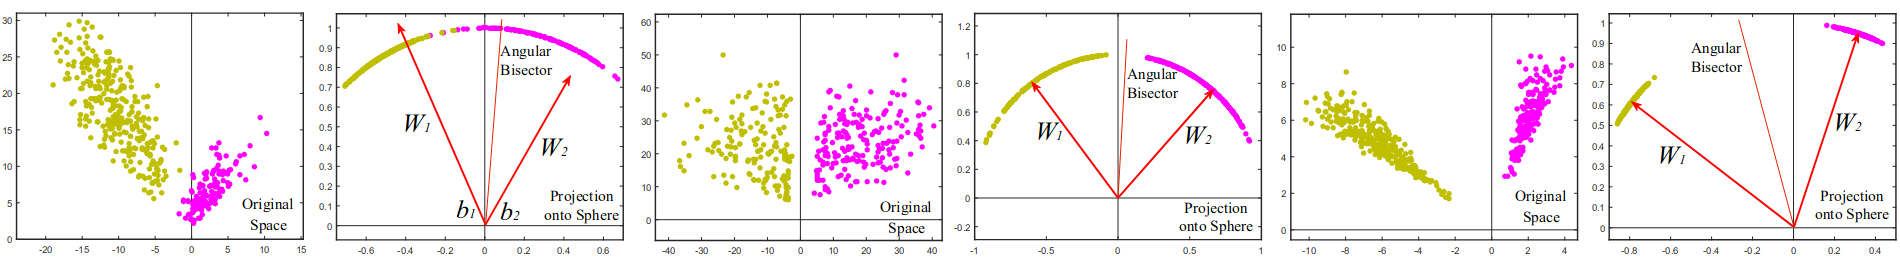
\includegraphics[scale=0.215]{sphereface.png}
    \caption{Comparison between the classic softmax loss, modified softmax loss (NormFace)~\autocite{wangNormFaceL2Hypersphere2017} and SphereFace \autocite{liuSphereFaceDeepHypersphere2018}.}
    \label{fig:sphereface}
\end{figure}

\vspace{0.7\baselineskip}
\noindent\textbf{$\rightarrow$ SphereFace (2018)}~\autocite{liuSphereFaceDeepHypersphere2018} improved the intra-class compactness and inter-class distance by introducing a very important concept of angular margin that contrasts with the usual Euclidean margin. As proven by Liu \textit{et al.}, features learned by softmax loss adopt an intrinsic angular distribution, therefore, euclidean margins are not compatible with softmax loss \reffig{fig:sphereface}. The decision boundary for a classic softmax loss function is $(W_1 - W_2)x+b_1-b_2=0$, and by normalizing the weights and zeroing the bias, it becomes $\|x\|(\cos{(\theta_1)}-\cos{(\theta_2)})=0$, where $x$ is a feature vector and the decision will only depend on the angles between class 1 and 2. SphereFace introduces the hyperparameter $m$ ($m\geq1 \in \mathbb{Z}$) that will, effectively, control the margin size between class 1 and 2 respectively as such $\|x\|(\cos{(m\theta_1)}-\cos{(\theta_2)})=0$ and $\|x\|(\cos{(\theta_1)}-\cos{(m\theta_2)})=0$.


\vspace{0.7\baselineskip}
\noindent\textbf{$\rightarrow$ AM-Softmax (2018)} and \textbf{CosFace (2018)} both improved SphereFace's main problem: the potential unstable training convergence due to the multiplicative angular margin. Thus, an additive cosine margin $\cos{\theta_{y_i}}+m$ is proposed to facilitate the convergence.

\begin{figure}[!h]
    \centering
    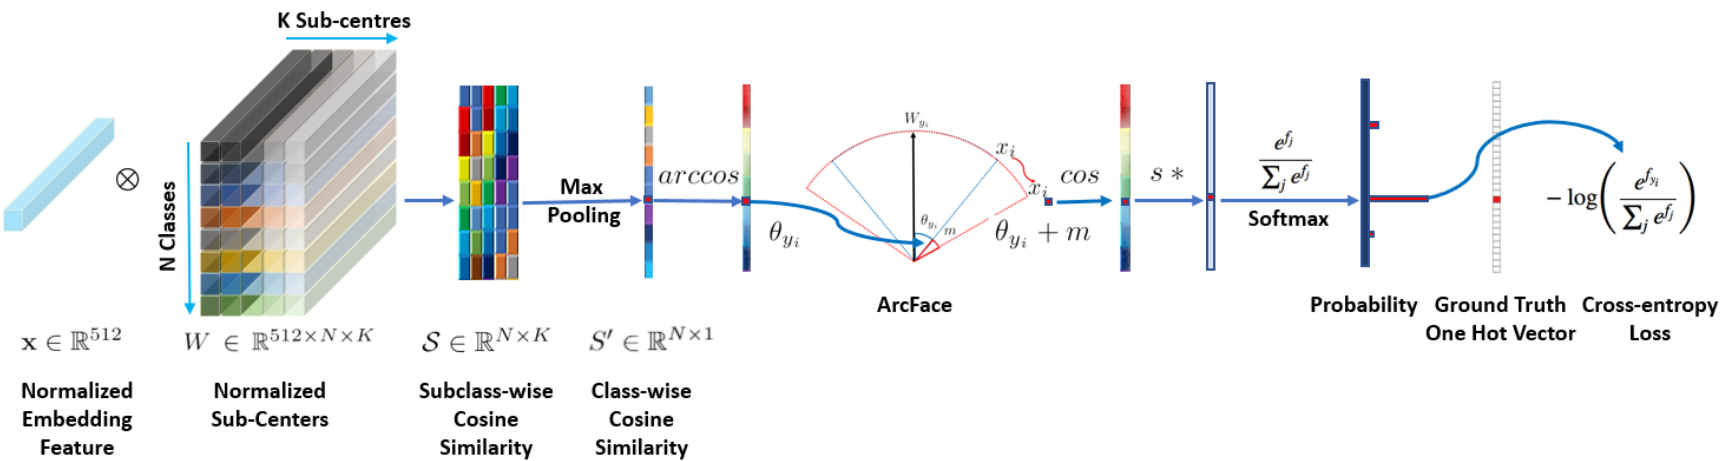
\includegraphics[scale=0.215]{arcface.png}
    \caption{ArcFace \autocite{dengArcFaceAdditiveAngular} training pipeline}
    \label{fig:sphereface}
\end{figure}

\vspace{0.7\baselineskip}
\noindent\textbf{$\rightarrow$ ArcFace (2019)}~\autocite{dengArcFaceAdditiveAngular} aims at optimizing the geodesic distance margin since there's a mathematical correspondence between the angle and the arc in the normalized hypersphere. Taking that into consideration, the cosine distance between features obtained by the dot product between the feature produced by the CNN and the fully connected layer, then arc-cosine is used to calculate the angle between the feature and the target one. Finally, the authors took the principles from AM-softmax \autocite{wangAdditiveMarginSoftmax2018} and SphereFace \autocite{liuSphereFaceDeepHypersphere2018} and introduced an additive angular margin directly to the angle $\cos{(\theta_{y_i}+m)}$, getting the target logit back by the cosine function and further stabilizing the training process and improving the discriminative power of the overall system. The loss function is reformulated by: 1) zeroing the bias and transforming the softmax loss logit $W^{T}_{j}x_i=\|W_j\|x_i\|\cos{(\theta_j)}$, as suggested in~\autocite{liuSphereFaceDeepHypersphere2018}, where $\theta_j$ is the angle between the weight $W_J$ and the feature $x_i$, 2) following~\autocite{wangNormFaceL2Hypersphere2017,liuSphereFaceDeepHypersphere2018,wangCosFaceLargeMargin2018} the weights are normalized by $L_2$, 3) the features $x$ are also normalized in $L_2$ per~\autocite{ranjanL2constrainedSoftmaxLoss2017,wangNormFaceL2Hypersphere2017,wangAdditiveMarginSoftmax2018,wangCosFaceLargeMargin2018} suggestion. This normalization insures that there's only an angular dependence between weights and features. By distributing the learned features through a hypersphere with radius $s$, and combining the margin penalties imposed by SphereFace~\autocite{liuSphereFaceDeepHypersphere2018}, CosFace~\autocite{wangCosFaceLargeMargin2018} and ArcFace, the geodesic distance can be optimized by the following unified framework:
\begin{equation}
\mathcal{L}=-\log\left(
                \frac{e^{s(\cos{(m_1\theta_{y_i}+m_2)-m_3})}}
                {e^{s(\cos{(m_1\theta_{y_i}+m_2)-m_3})} + \sum_{j=1, j\neq y_i}^{N}e^{s \cos{(\theta_j)}}}
            \right),
\end{equation}
\noindent where $m_1$, $m_2$ and $m_3$ are the hyperparameters relating, respectively, to SphereFace, ArcFace and CosFace.

\vspace{\baselineskip}
To this day, ArcFace is still the state-of-the-art regarding face recognition, and one of the most implemented loss functions of this category, consequently, it is usual to see other novel cost functions to try to improve it by using it as a base foundation to other tasks. The accuracy saturation of more common benchmarks like LFW~\autocite{huangLabeledFacesWild} lead to the appearance of harder ones, namely XQLFW~\autocite{knocheCrossQualityLFWDatabase2021} or IJB-S~\autocite{kalkaIJBIARPAJanus2018}, which by itself, ultimately, lead to loss functions aimed at more specific challenges, namely CurricularFace~\autocite{huangCurricularFaceAdaptiveCurriculum2020}, MagFace~\autocite{mengMagFaceUniversalRepresentation2021}, AdaFace~\autocite{kimAdaFaceQualityAdaptive2022} or QMagFace~\autocite{terhorstQMagFaceSimpleAccurate2023}.

\subsubsection{Metric learning loss functions}
Metric learning loss functions include the methods that aim optimizing the distance between feature embeddings. That is, increase the distance between negative embeddings and minimize the distance for those that are positive.
\par One classic example is the contrastive loss, but this category's attention mainly pends over the triplet loss first implemented by Schroff \textit{et al.} in FaceNet~\autocite{schroffFaceNetUnifiedEmbedding2015}. 

\vspace{0.7\baselineskip}
\noindent\textbf{$\rightarrow$ Contrastive Loss}~\autocite{duElementsEndtoendDeep2022} has the objective of optimizing the distance between identity pairs: positive pairs are encouraged to be closer and negative ones to be further apart. The loss function to be minimized is

\begin{equation}
    \mathcal{L}_{contrastive} = 
    \begin{cases}
      \frac{1}{2}\|f(x_i)-f(x_j)\|^{2}_{2}, \text{if} y_i=y_j\\
      \frac{1}{2}\max{(0, m_d-\|f(x_i)-f(x_j)\|_2)^2}, \text{if} y_i\neq y_j
    \end{cases}
\end{equation}

\begin{figure}[!h]
    \centering
    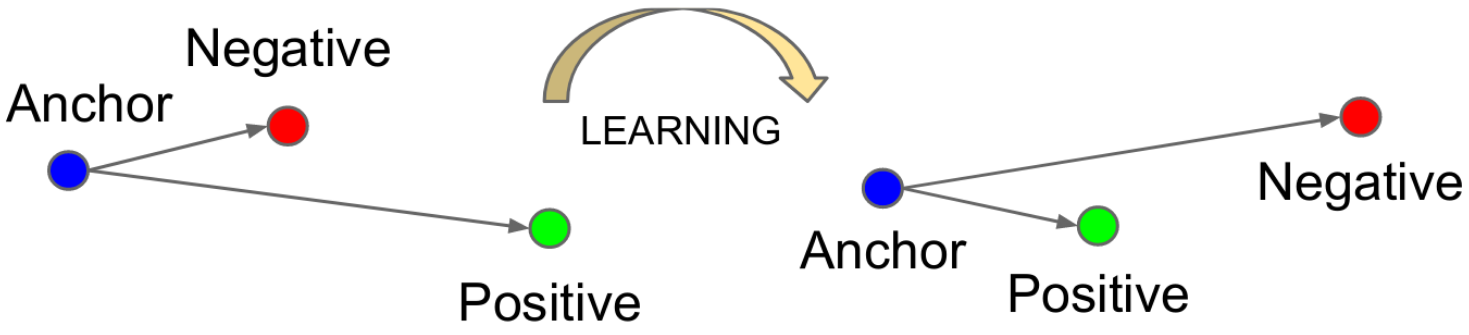
\includegraphics[scale=0.215]{triplet.png}
    \caption{Triplet}
    \label{fig:triplet}
\end{figure}

\vspace{0.7\baselineskip}
\noindent\textbf{$\rightarrow$ Triplet Loss (2014)}~\autocite{schroffFaceNetUnifiedEmbedding2015} embeds an image to a d-dimensional feature vector in an Euclidean space. The motivation is to guarantee that, for every individual $i$, the squared distance between an image $x^{a}_{i}$ (anchor) of an identity and its corresponding true identities $x^{p}_{i}$ (positive) is smaller than the distance between non-identities, $x^{n}_{i}$ (negative). This structure is called a triplet \reffig{fig:triplet}. The aforesaid can be described in mathematical terms as:
\begin{equation}
\|f(x^{a}_{i})-f(x^{p}_{i})\|^{2}_{2} + \alpha < \|f(x^{a}_{i})-f(x^{n}_{i})\|^{2}_{2},
\end{equation}

\noindent where $f(\dot)$ are the feature embeddings from all the possible triplets, and $\alpha$ is a margin between positive and negative pairs. Therefore, the loss function to be optimized is:
\begin{equation}
\mathcal{L}_{triplet} = \sum_{i}^{N}\left[\|f(x^{a}_{i})-f(x^{p}_{i})\|^{2}_{2}-\|f(x^{a}_{i})-f(x^{n}_{i})\|^{2}_{2}+\alpha\right]
\end{equation}

However, there's a major drawback associated with this methodology. The selection of the triplets are essential for good results and there's a combinatorial explosion regarding the number of possible triplets, specially for large-scale datasets, leading to a slower convergence and computational overhead if all the possible triplets are to be used. The only way to address this problem is through the development of efficient mining strategies that select both hard and representative triplets.

\section{Related work}
\label{sec:related_work}
The development of solutions for student monitoring has encompassed a plethora of possibilities. Depending on the application, they can be intended for commercial purposes or developed as part of academic research. Commercial solutions such as Kryterion, ProctorExam, ProctorU, Procotorio, ProctorFree, or SMOWL~\autocite{labayenOnlineStudentAuthentication2021} are available; however, with the exception of SMOWL, due to their proprietary nature, their methods of implementation are not disclosed, making it impossible to study them adequately. Therefore, all the methods analyzed, other than SMOWL, will fall under the second category.

\vspace{0.7\baselineskip}
\noindent\textbf{$\rightarrow$ Zhang \textit{et al.}~\autocite{zhangVirtualLaboratorySystem2016} (2016)} studied a system based on facial features exclusively. The faces are first detected and extracted using the OpenCV pretrained classifier based on the Viola-Jones/Haar Cascades algorithm. Subsequently, recognition is carried out utilizing the Eigenfaces algorithm, which incorporates Principal Component Analysis (PCA). The main disadvantage of this solution is lacking the flexibility to adverse visual conditions that Deep Learning techniques have.

\vspace{0.7\baselineskip}
\noindent\textbf{$\rightarrow$ Atoum \textit{et al.}~\autocite{atoumAutomatedOnlineExam2017} (2017)} proposed a solution that employs Viola-Jones/Haar Cascades face detector and Minimum Average Correlation Energy (MACE) filter for face verification. Once again, the methodologies utilized are too sensitive to image variations, such as illumination, pose, expressions, etc.

\vspace{0.7\baselineskip}
\noindent\textbf{$\rightarrow$ Zhang \textit{et al.}~\autocite{zhangVirtualProctorBiometric2018} (2018)} latter proposed another solution. In a similar fashion to Zhang \textit{et al.}~\autocite{zhangVirtualLaboratorySystem2016} and Atoum \textit{et al.}~\autocite{atoumAutomatedOnlineExam2017}, the face detection is achieved through the same OpenCV pretrained module. On the other hand, the detected and cropped faces are now processed by a modification of the Stereo Matching algorithm. Because this method extracts information from pairs of stereo images, it is subject to occlusions, ambiguities, textures, etc.

\vspace{0.7\baselineskip}
\noindent\textbf{$\rightarrow$ Sawhney \textit{et al.}~\autocite{sawhneyRealTimeSmartAttendance2019} (2019)} introduced an approach where the face detection is accomplished in two stages: 1) bounding box regression with the Viola-Jones/Haar Cascades algorithm and 2) facial landmark generation with a Local Model-based algorithm. After the faces are extracted, the face recognition stage, in similarity with Zhang \textit{et al.}~\autocite{zhangVirtualLaboratorySystem2016}, applies simultaneously Eigenfaces with PCA, therefore, the drawbacks coincide.


\vspace{0.7\baselineskip}
\noindent\textbf{$\rightarrow$ Ganidisastra and Bandung~\autocite{ganidisastraIncrementalTrainingDeep2021} (2021)} introduced a Deep Learning-based approach that employs two models for face detection and recognition: YOLO-face for face detection and Facenet for face recognition. Notably, Facenet is continuously trained with data collected at the end of each user session. This training process causes the system to overfit to each individual identity, leading to reduced adaptability in handling new scenarios due to limited data availability. Furthermore, the training of Facenet utilizes the triplet loss, which can be computationally challenging, especially on less powerful hardware. This is primarily due to the exponential increase in possible combinations when mining triplets during the training process.

\vspace{0.7\baselineskip}
\noindent\textbf{$\rightarrow$ SMOWL~\autocite{labayenOnlineStudentAuthentication2021} (2021)} is a multi-modal tool that analyzes voice, face and key-strokes data. For this dissertation, the interest resides only on the facial aspect of it. For face detection, it utilizes a combination of FaceBoxes with MobileNet-SSD for occlusion detection. The face recognition is accomplished with a Facenet model trained with triplet loss on the MS-Celeb-1M dataset. Anew, the triplet loss training can be considered a drawback. 

\vspace{0.7\baselineskip}
\noindent\textbf{$\rightarrow$ TrustID~\autocite{fariaImagebasedFaceVerification2023} (2023)} is our solution, designed and developed at ISR - Instituto de Sistemas e Robótica from University of Coimbra. It utilizes as a face detection a linear detector conjointly with a Histogram of Oriented Gradients and pyramidal image search. After the faces are detected and aligned, they're cropped to a Region of Interest (RoI) of $150\times150$ pixels. Finally, the faces are passed to a face recognition that uses a CNN called ResNet-34, trained with triplet loss on a dataset of, approximately, 3 million faces derived from the Visual Geometry Group
Face~\autocite{parkhiDeepFaceRecognition2015} and FaceScrub~\autocite{ngDatadrivenApproachCleaning2014} datasets.


\vspace{\baselineskip}
\par As stated before, the choice of architecture will be based only on Deep Learning approaches. That is, because the system will be deployed on a difficult scenario where control of, more specifically, illumination, pose and quality will be impossible. Henceforth, a framework insensitive to those variations is the correct choice.

\end{document}